\documentclass[article,twocolumn,preprint,10pt]{paper}%{revtex4-1}

\usepackage{epsfig,graphicx,amsmath}
\usepackage{amsfonts,amssymb,amsthm}
\usepackage{enumerate}
\usepackage{epstopdf}
\usepackage{afterpage}
\usepackage{color}

\usepackage[caption=false]{subfig}
\newcommand{\nn}{\nonumber}
\newcommand{\ba}{\bea \begin{array}}
\newcommand{\ea}{\end{array} \eea}
\renewcommand{\(}{\left(}
\renewcommand{\)}{\right)}
\renewcommand{\[}{\left[}
\renewcommand{\]}{\right]}
\newcommand{\bc}{\begin{center}}
\newcommand{\ec}{\end{center}}
\newcommand{\p}{\partial}
\newcommand{\cb}{\mbox{\boldmath$c$}}

\newcommand{\red}{\textcolor{red}}
\newcommand{\blue}{\textcolor{blue}}
\newcommand{\mb}[1]{ \mbox{\boldmath$#1$}}
\newcommand{\ds}{\displaystyle}
\newcommand{\beq}{\begin{eqnarray}}
\newcommand{\eeq}{\end{eqnarray}}
\newcommand{\beqq}{\begin{eqnarray*}}
	\newcommand{\eeqq}{\end{eqnarray*}}
\newtheorem{thm}{Theorem}[section]


\newcommand{\g}{\gamma}
\newcommand{\epsv}{\epsilon}
\newcommand{\eps}{\varepsilon}
\newcommand{\oln}{\overline }

\newcommand{\Om}{\mbox{\boldmath$\omega$}}
\newcommand{\x}{\mbox{\boldmath$x$}}
\newcommand{\U}{\mbox{\boldmath$U$}}
\newcommand{\V}{\mbox{\boldmath$V$}}
\newcommand{\R}{\mbox{\boldmath$R$}}
\newcommand{\E}{\mbox{\boldmath$\eta$}}
\newcommand{\Id}{\mbox{\boldmath$I_d$}}
\newcommand{\M}{\mbox{\boldmath$M$}}
\newcommand{\N}{\mbox{\boldmath$N$}}
\newcommand{\1}{\mbox{\boldmath$1$}}
\newcommand{\hx}{\mbox{$\hat x$}}
\newcommand{\n}{\mbox{\boldmath$n$}}
\newcommand{\J}{\mbox{\boldmath$J$}}
\newcommand{\y}{\mbox{\boldmath$y$}}
\newcommand{\z}{\mbox{\boldmath$z$}}
\newcommand{\bt}{\mbox{\boldmath$\beta$}}
\newcommand{\tb}{\mbox{\boldmath$t$}}
\newcommand{\ic}{\mathtt{i_c}}
\newcommand{\di}{\text{d}}

\font\bb=msbm10 at 12pt \font\bbbis=msbm10 at 10pt
\def\bz{\bar{z}}
\def\rR{\hbox{\bb R}} \def\nN{\hbox{\bb N}}
\def\rRp{\hbox{\bbbis R}} \def\nN{\hbox{\bb N}}
\def\zZ{\hbox{\bb Z}} \def\qQ{\hbox{\bb Q}}
\def\cC{\hbox{\bb C}} \def\sS{\hbox{\bb S}}
\def\pP{\hbox{\bb P}}

\newcommand{\vect}[1]{\boldsymbol{#1}}


%%%%%%%%%%%%%%%%%%%%%%%%%%%%%%%%%%%%%%%%%%
\begin{document}
	\title{Machine learning framework for correcting the prediction of the IOL power by second and third generation formulas\\}
    \author{Ofir Shukron, Jacky Hochner, Michael Assoline MD\\Mikajaki}
	\maketitle
	\section{Highlights}
	\begin{enumerate}
		\item We develop a method to correct the IOL power from Gaussian optics formulas  (second and third generation) to arrive more closely to target refraction post-op;
		\item We achieve 60\% accuracy in predicting refractive errors below 0.25D, and 80\% below 0.5D. 
		\item We achieve 85\% accuracy in predicting the IOL formula, which produces the lowest refractive error.
	\end{enumerate}

	\begin{abstract}
		In this work we develop a framework composed of a combination of regressors and a machine-learning classifier, to predict the IOL power to be implanted in order to arrive at target refraction. We demonstrate our methodology on a dataset of 1397 cataract surgery records. We derive a relationship between the correction to the power predicted from formulas and the expected refraction error based on Gaussian optics for seven IOL formulas. We further train a classifier to automatically select the formula which will produce the smallest error from target refraction post op. Our classifier relies on objective measurements from the IOL-master, and operates without the need to introduce any fudge factors and approximations in formulas. We find that an average of -0.5D needs to be subtracted from IOL formula to arrive more closely to target refraction. The mean absolute error of out predictors was 0.3D after classification. We thus demonstrate that our methodology is accurate and applicable in all the range of biophysical parameter, accounting for both short and long eyes in a one homogeneous framework.  Our presented methodology can be adapted to clinic-specific practices and is easy to implement and operate in real-time.
	\end{abstract}

\section{Introduction}\label{section:introduction}
Intraocular lens (IOL) implantation to replace cataracteous lens requires the computation of the power of the artificial lens to achieve target refraction. Over the past half a century, various formulas were developed to assist in the computation of the IOL power, based on patient-specific biophisical measurements, such as the axial length and the anterior chamber depth (ACD). Those formulas have progressively evolved in complexity and accuracy, and were thus accordingly grouped into generations. Starting with first generation formulas, which rely primarily on empirical regression methodologies, such as the SRK formula (\cite{retzlaff1990}, \cite{sanders1980}), Fyodorov, Hoffer Colenbrander and Van der Heijde.  Over time, IOL formulas were derived by model-based approach, utilizing a simplified eye model and Gaussian optics in the paraxial approximation \cite{retzlaff1990, Haigis, Olsen} \cite{Barrett-1,Barrett-2} (second generation). Third Generation formulas include a combination of model-based, Gaussian optics, and regression methodologies to assess parameters \cite{retzlaff1990}. Other authors attempted at including the lens design into theoretical formula, which resulted in improved prediction over 3rd generation formulas \cite{naeser1997}. More recent advancement in IOL prediction included theoretical derivations and simulated ray-tracing algorithms \cite{Okulix}. Whereas other methodologies harnessed the power of machine learning (ML) to predict the IOL power, such as the Hill RBF-kernel \cite{} and the Ladas super formula \cite{ladas2015}. Regression method still persists to this day, with more modern regression formula for toric IOL lenses \cite{abulafia2016}.

While all computational methodologies were shown to well predict the IOL power and final refraction for some range of the biophysical parameter domain, e.g. either for long or short eyes, none of the formulas ws proven to satisfy the whole range. Over time, attempts were made to create rules of thumb to the use of one or another formula, depending on the objective measurement of a patient. 

A prediction of the IOL power which results in obtaining post-operative target refraction is met with challenges of three main sources: (1) model error- the use of inaccurate modeling to predict the post-operative effective lens position (ELP) in various advanced formulas (2) practice errors- stemming from surgeons practices during surgery, and (3) measurement error pre-surgery, which might result in errors of the predicted power even when  the most advanced IOL formula is used. 
A possible fourth source of errors stems from inherent inability of a given formula to accurately predict IOL power in the full range of physical eye parameters, such as the axial length. To overcome such difficulty, fudge factors and rules of thumb were made to aid physician select the formula best fit based on patient specific-measurements. It is thus left as a surgeon judgment and experience to decide on the use of an adequate formula based on patient-specific pre-operational measurements. Several formulas are reported to be more accurate for short eyes, whereas others  are reported to be more accurate for long eyes. For average eyes, the majority of high generation formulas perform equally well. It thus, remains a surgeon practice to choose among several formulas which works best in their clinical practice. 

The major difference between formula based on Gaussian optics, is in the manner in which their authors estimate model parameters. Specifically, various authors have argued for the need to use a post-op value for axial length and ELP. In addition, the lens material and surgeon-specific  practices are taken into account using the so called lens A-constant, which in turn affect the estimation of these two key parameters. Other differences between formula stem from the estimation of the refractive indices of the cornea, and are estimated either according to thick or thin lens heuristics. Despite the advancement in modeling approach, some of the aforementioned parameters are still estimated using regression methodologies, and are therefore non-universal and database dependent. These variations reflected in the quality of data gathered in each clinic, then necessitate update of those key parameters, and specifically the A constant (or surgeon constant) in a clinic-specific manner. 

A comparison of the performance of formulas, in the sense of their ability to predict the final refraction post-op, encounters several sources of errors. The first, is the time in which the visual acuity (VA) measurement is performed post op., which can affect recorded VA over successive measurements. The second, is the difference between the predicted ELP and the actual end position of the artificial lens. The latter also depends somewhat on the time and equipment used to determine the ELP post-op. In addition, the comparison of the final refraction (VA) is done by back-calculating the final refraction based on the actual IOL power implanted. This means, inserting the IOL power implanted into a given equation, to retrieve refraction. 

A lens that supplies a power to achieve target refraction might not exist in practice, and therefore a residual refraction error is present. If such IOL power would have existed, there would expect to see no difference between the IOL formulas in terms of the MAE, because target refraction should equal predicted refraction. It is therefore, that what differentiate formulas primarily stems from the relationship between the power difference (implanted-predicted) and the final refraction difference (measured-predicted), given the parameters estimated. Lastly, physician working with a given formula, have empirically found the power difference between that predicted by the formula that needs to be implanted to arrive as close as possible to target refraction. It implies then that the power suggested by a given formula might not be implanted in practice, which make the comparison of formulas more complex. 

In this work, we present a unified framework to predict the IOL power, allowing an automatic choice of the most adequate formula based on patient-specific measurements. We present our construction of a machine-learning predictor of formula, rather than predicting the IOL power, as is the approach taken by other authors. Our Machine-learning framework, thus alleviates the need to select a formula or introduce any fudge factors. We show that our method outperform all currently implemented formulas, in terms of accuracy of IOL power predicted vs IOL power implanted. 

%%%%%%%%%%%%%%%%%%%%%%%%%%%%%%%%%%%%%%%%%%
\section{Methods}\label{section:Methods}
Below we describe the computational procedure to predict refractive error for each IOL formula. 
\subsection{Predicting the refractive error}\label{subsection:predictingRefractiveError}
In this study we use the following IOL formulas
\begin{enumerate}
	\item SRK/T;
	\item Shammas;
	\item Haigis;
	\item Binkhorst-2;
	\item Holladay-1;
	\item Hoffer-Q;
	\item Olsen.
\end{enumerate} 
Details of the implementation of IOL formulas appear in the Appendix (Section \ref{section:iolFormulas}). We implemented all formulas according to the descriptions in their original articles. All IOL formulas were computed with a lens A-constant of 118.9. 
All the IOL formulas used in this study are derived from the Gaussian optics formula in the paraxial approximation. We note below the two equation for the IOL power $P$ and the expected refraction $R$ (unless specified otherwise by authors of formulas, in which case we implement the suggested refraction as presented in their original articles):
\beq 
P &=& \frac{n_v}{L-e} - \frac{n_c}{\frac{n_c}{K+R_t}-e },\label{eq:expectedPower}\\
R &=& \frac{n_c}{\frac{n_c}{\frac{n_v}{L-e}-P_i}+e}-K,\label{eq:expectedRefraction}
\eeq 
where $n_c$ is the refractive index of the cornea, $n_v$ is the refractive index of the aqueous media, $L$ is the axial length (mm), $K$ is the mean keratometry (D), $e$ is the effective lens position (ELP) in mm, $P_i$ is the IOL power implanted (D), and $R_t$ is the target refraction (D).

In theory, all IOL formulas should produce the exact same mean absolute error (MAE) between target refraction $R_t$ and final refraction $R$ (visual acuity), which can only be obtained when $P_i= P $. However, in practice, $P\neq P_i$, as the theoretical IOL power as predicted from a given formula (Eq. \ref{eq:expectedPower}), do not currently exist in the market, and IOL powers are  available primarily in intervals of 0.5D. The expected refraction $R$, therefore, is  computed by inverting the Gaussian optics formula (Eq. \ref{eq:expectedPower}) to obtain Eq. \ref{eq:expectedRefraction}, and using the rounded IOL power $P_i$  as a parameter.
As market available IOL power will be supplied in smaller dioptric intervals, so would the expected refraction $R$ converge to $R_t$, and hence all formulas will produce the exact same MAE. 
It is, therefore, that the method to rank formulas based on expected refraction is only expresses the sensitivity of refraction to change of available IOL power (after rounding). We find this approach to be inaccurate. 
Instead, we adopt here a different approach, in which we directly predict the refraction error $\Delta R = R_f-R_t$, using patient-specific biophysical parameters of the eye, where $R_f$ is the subjective visual acuity op op. We then use the predicted $\Delta R$ to correct the power  computed from each formula, such that the power implanted will produce final refraction closer to the target refraction. 
To predict $\Delta R$, we first establish a theoretical relationship between the change in IOL power $\Delta P=P_i-P$ and $\Delta R $ 
\beq \label{eq:dPvsDR}
\Delta P = \frac{-n_c^2\Delta R}{\alpha^2 -e\alpha\Delta R},
\eeq 
where 
\beq 
\alpha &=& n_c-e(K+R_t)\nonumber 
\eeq 
with $e$ is the ELP (mm). Details of the derivation of Eq. \ref{eq:dPvsDR} appear in the Appendix (subsection \ref{subsection:derivationOfdPTodR}).
We use the relationship in Eq. \ref{eq:dPvsDR} to obtain the required correction $\Delta P$ to the predicted  IOL power $P$ in Eq. \ref{eq:expectedPower}. This will allow us to obtain a corrected IOL power $P_{corr}$ to arrive more closely to the target refraction for any formula based on the Gaussian optics. The adjustment to the IOL power is computed by
\beq \label{eq:correctedPower}
P_{corr} = P+\Delta P.
\eeq 
where $P$ is the power predicted from a given formula to reach target refraction, and $\Delta P$ is computed by Eq. \ref{eq:dPvsDR} given a predicted $\Delta R$. The prediction of $\Delta R$ will be performed by regression. 

\subsubsection{Training and validating regressors}\label{subsection:regressorsTrainingAndValidation}

To compute $\Delta P$ in Eq.\ref{eq:correctedPower}, we train a linear regressor to first predict $\Delta R$, and  then use the predicted $\Delta R$ as a parameter in Eq. \ref{eq:dPvsDR} to obtain $\Delta P$. 
For this end,  we use the database of retrospective patient data,  and fit a liner regressor for $\Delta R$ using RANSAC methodology. Features used for the fitting procedures are: Age (year), $\bar{K}$ (D), ACD (mm), $L$ (mm), $R_t$ (D).
Each IOL formula used in this study (see list in subsection \ref{subsection:predictingRefractiveError}) suggests a specific adjustment to the axial length $L$, values for the refraction indices $N_c, n_v$, and further provides a specific prediction of the ELP $e$. We, therefore, use formula-specific parameters in the regressor training procedure. We note, that the estimation of both the axial length and the ELP are independent of the target refraction $R_t$ and power $P$ for all formulas in this study. 
We set a threshold for inliers of $T=0.5$ for the RANSAC regression, and define a costume loss for to compute for each iteration, given by 
\beq 
loss = \begin{cases}
	0, &|R-R_f|\leq 0.25\\
	\frac{T}{2}, & 0.25<|R-R_f|\leq 0.5\\
	1 & |R-R_f|>0.5
\end{cases}
\eeq 
an 85\% for the minimal number of samples chosen randomly from the original data. 
observations with loss>T are discarded from the random consensus in each iteration.
 
We  use 85\% of our database for training, leaving 15\% for validation. Training and validation sets were chosen uniformly at randomly. To validate the accuracy of our regressors, we compute the cumulative absolute error $E_{reg}(\delta)$ at $\delta =[0, 0.25D, 0.5,D, 0.75D, 1D]$ from observed refraction error $\delta R_o$, i.e. we compute 
\beq \label{eq:regressionCumError}
E_{reg}(\delta) = \sum_{i=1}^NH(|\Delta_i R -\Delta_i R_o|- \delta )
\eeq 
with 
\beq \label{eq:Hfunction}
H(x)=\begin{cases}
	1, & x\leq 0\\
	0, & x>0
\end{cases}
\eeq 
for $\delta\in [0,0.25, 0.5, 0.75,1]$.

\subsection{Constructing a classifier for IOL formulas}\label{subsection:ClassificationOfIOLFormulas}
In addition to fitting regressor each IOL formula, we set out to construct a classifier to automatically select the best regressor (IOL formula), for each set of objective patient measurement. A mechanism automatic selecting the IOL formula provides means to overcome empirical rules of thumb in selecting the best formula in different ranges of patient objective measurements (i.e. long or very short axial length). For this end, we chose to use the K nearest-neighbors (KNN) classifier  due to its simplicity and after empirically verifying that it performs equally well as other more complex methodologies (e.g. random forest, SVM, etc).
Features used for training the KNN classifier are: pre op $L$, pre op $ACD$, $\bar{K}$, and $R_t$. We emphasize here that the $ACD$ and $L$ are taken from pre op. objective measurements and are not the adjusted values, as in the case of training regressors (see \ref{subsection:regressorsTrainingAndValidation}).
We enumerate each regressor by an integer number (class) according to their order of appearance in the list of IOL formulas in this study (see list in \ref{subsection:predictingRefractiveError}). We assign a ground-truth class label $\mathcal{C}_i$ for each observation $i=1\ldots N$ in the training and validation set, as the regressor number which produces the minimal value for $\ds \mathcal{C}_i =  argmin_{j=1\ldots 7} |\Delta R-\Delta R_o|_j$, where we round the $\Delta R$ and $\Delta R_o$ to the nearest quarter of diopter.

To tune model hyperparameters we use grid search methodology with cross-validation. We devise a model scoring function $CV_score$ for cross-validation, which favors a classifier parameters that predicts $\delta R$ within the range of 0.25D from observed $\delta R_o$.  i.e. the cross-validation score is given by 
\beq 
CV-score = \sum_{i=1}^{N_{cv}}H(|\Delta_{\mathcal{C}_i} R - \Delta_i R_o|-0.25)
\eeq 
where $H(\delta)$ is defined in Eq. \ref{eq:Hfunction},  $N_{cv}$ is the number of observations in each fold of the cross-validation (higher score is better), and $\Delta_i R$ is the $i^{th}$ refraction error.
 
We compute the accuracy of classification on the validation set as the percentage of correct class assignment set for which predicted class equaled the ground truth label. However, because several regressor can achieve similar refraction error after rounding the predicted $\Delta R$ to the nearest quarter of dipoter.

\subsubsection{Computational tools}
All codes were written in Python 3.8. All computations were performed by an in-house codes. Machine learning, classification and optimization were performed by the python sklearn toolset.


\section{Results}
Data in this study consists of 1387 eye records from Clinique Iena Vision (CIV), Paris France acquired between the years 2011 and 2020. Patient measurement prior to surgery consisted of IOLmaster (Zeiss), and are referred to hereafter as objective measurements. 
Inclusion criteria for patients in this study appear in Table \ref{Table: inclusionCriteria}. 
\begin{table}
	\begin{tabular}{l|c|}
		Parameter & Range [min, max] \\
		\hline  
		Age (years)  & [40,100]\\
		$\bar{K}$ (D)& [35,47]\\
		Axial length (mm)  & [20,40]\\
		ACD (mm) & [2,5]\\
		WTW (mm) & [10,13]\\
		Target refraction (D) & [-10,10]\\
		Followup (days) & [10,90]
	\end{tabular}
	\label{Table: inclusionCriteria}
	\caption{Inclusion criteria for patients in this study.}
\end{table}
Mean keratometry was computed from the mean cornea radius (mm) using refraction index of 1.336. In addition to objective measurements, we extract from the electronic medical record (EMR) the IOL power implanted $P_i$, the implant types, and the final refraction $R_f$ (sphere only) as the subjective visual acuity post surgery performed at follow-up session.

In Table \ref{table:summaryStatistics} we provide summary statistics for objective measurements in this study.
\begin{table}
	\begin{tabular}{l|c|c|c|c}
		parameter	   	&mean& std& min& max \\
		\hline 
		\hline
		age           & 71.00   & 8.83  & 40.73 & 97.58\\
		$\bar{k}$  & 43.53  & 1.51   & 36.01  & 47.00\\
		$L$           & 23.88  & 1.38  & 20.12  & 30.17\\
		$ACD$	   & 3.12    & 0.40  & 2.10    & 4.78\\
		$WTW$ 	 & 11.87   & 0.39  & 10.70  & 13.50\\
		$R_t$	    & -0.31   & 0.57  & -3.0    & 1.00 \\		
	\end{tabular} 
	\caption{Summary statistics of 1387 eyes undergoing cataract surgery used in this research. $\bar{k}$- mean keratometry (D), $L$- axial length (mm), ACD- anterior chamber depth (mm), WTW- white to white (mm), $R_t$- target refraction (D).}
	\label{table:summaryStatistics}
\end{table}
\subsubsection{ IOL power predicted differs from implanted in the majority of cases}
At the site of data collection, the SRK/T formula was predominantly used in pre-surgery planning stage, covering 99.5\% of the cases. The power implanted $P_i$ and the power predicted  $P$ by the SRKT formula differed in the majority of cases, with only 22\% of cases (308) where $P=P_i$,  36\% (496) of cases where the power differed by $\pm 0.5$D, 21\% (297) of cases the power differed by $\pm1$D, 10.5\% (146) where the power differed by $\pm1.5$D, and in 9.5\% (127) the power differed by at least $\pm2$D. 
The mean difference between the power implanted $P_i$  and the power predicted $P$ by SRK/T was -0.51D (absolute difference 0.81D), indicating surgeon-specific decision to subtract an average of $\Delta P=-0.5D$ from he predicted power to arrive at target refraction post op. 
The MAE between target refraction $R_t$ and the final subjective refraction $R_f$ (VA) was 0.55D, showing that residual refraction error remains even after surgeon's adjustment of the IOL power. We thus concentrate here on the automatically predicting the iol power correction $\Delta P$ to arrive more closely at target refraction post op. which allows us to free physicians from empirical rules of thumb to adjust the IOL power and provide correction to IOL formulas. 

\subsection{ Mean absolute refraction  error conditional on the power implanted}
Fromthe retrospective database, we set out to estimate the accuracy of formulas in predicting the final refraction given the power implanted. For this end we first computed $R$ from Eq. \ref{eq:expectedRefraction} for each formula, where we used the power implanted $P_i$  and formula-specific axial length and predicted ELP in the respective formulas, and the computed the MAE for refraction predicted vs final post op refraction. We rounded the resulting predicted refraction to the nearest quarter of diopter. In Fig. \ref{fig:cumulativeRefractionError_powerImplanted} we present the cumulative refraction error at ranges of 0 to 1D. From Fig. \ref{fig:cumulativeRefractionError_powerImplanted} we appreciate that the Haigis formula would have been more predictive of the final observed refraction given the power implanted, than any other formulas used in this study, with 40\% of observations below 0.25 error, 60\% below 0.5D, and 76\% below 0.75D. The SRKT formula,  which was predominantly used in the clinic where data was collected, obtained conditional refraction error with 30\% of observations below 0.25D, 45\% below 0.5D, and 60\% below 0.75D. However, had the Haigis formula  been used in surgery planning stage, the power implanted might have differed than that finally recorded. 
The MAE of formulas given the power implanted were: SRK/T 0.82D, Shammas 0.73D, Haigis 0.63D, Hoffer-Q 1.4D, and Holladay-1 0.7D. The Olsen and Binkhorst-2 formulas average predicted ELP was 3mm, which was nearly half that predicted by other formulas (average 5.5mm). This difference in the predicted ELP constituted the large difference in the MAE between Olsen and Binkhorst-2 and the reminder of the formulas. Indeed, the MAE for Olsen and Binkhorst-2 conditional on $P_i$ were 3D. 

\begin{figure}
	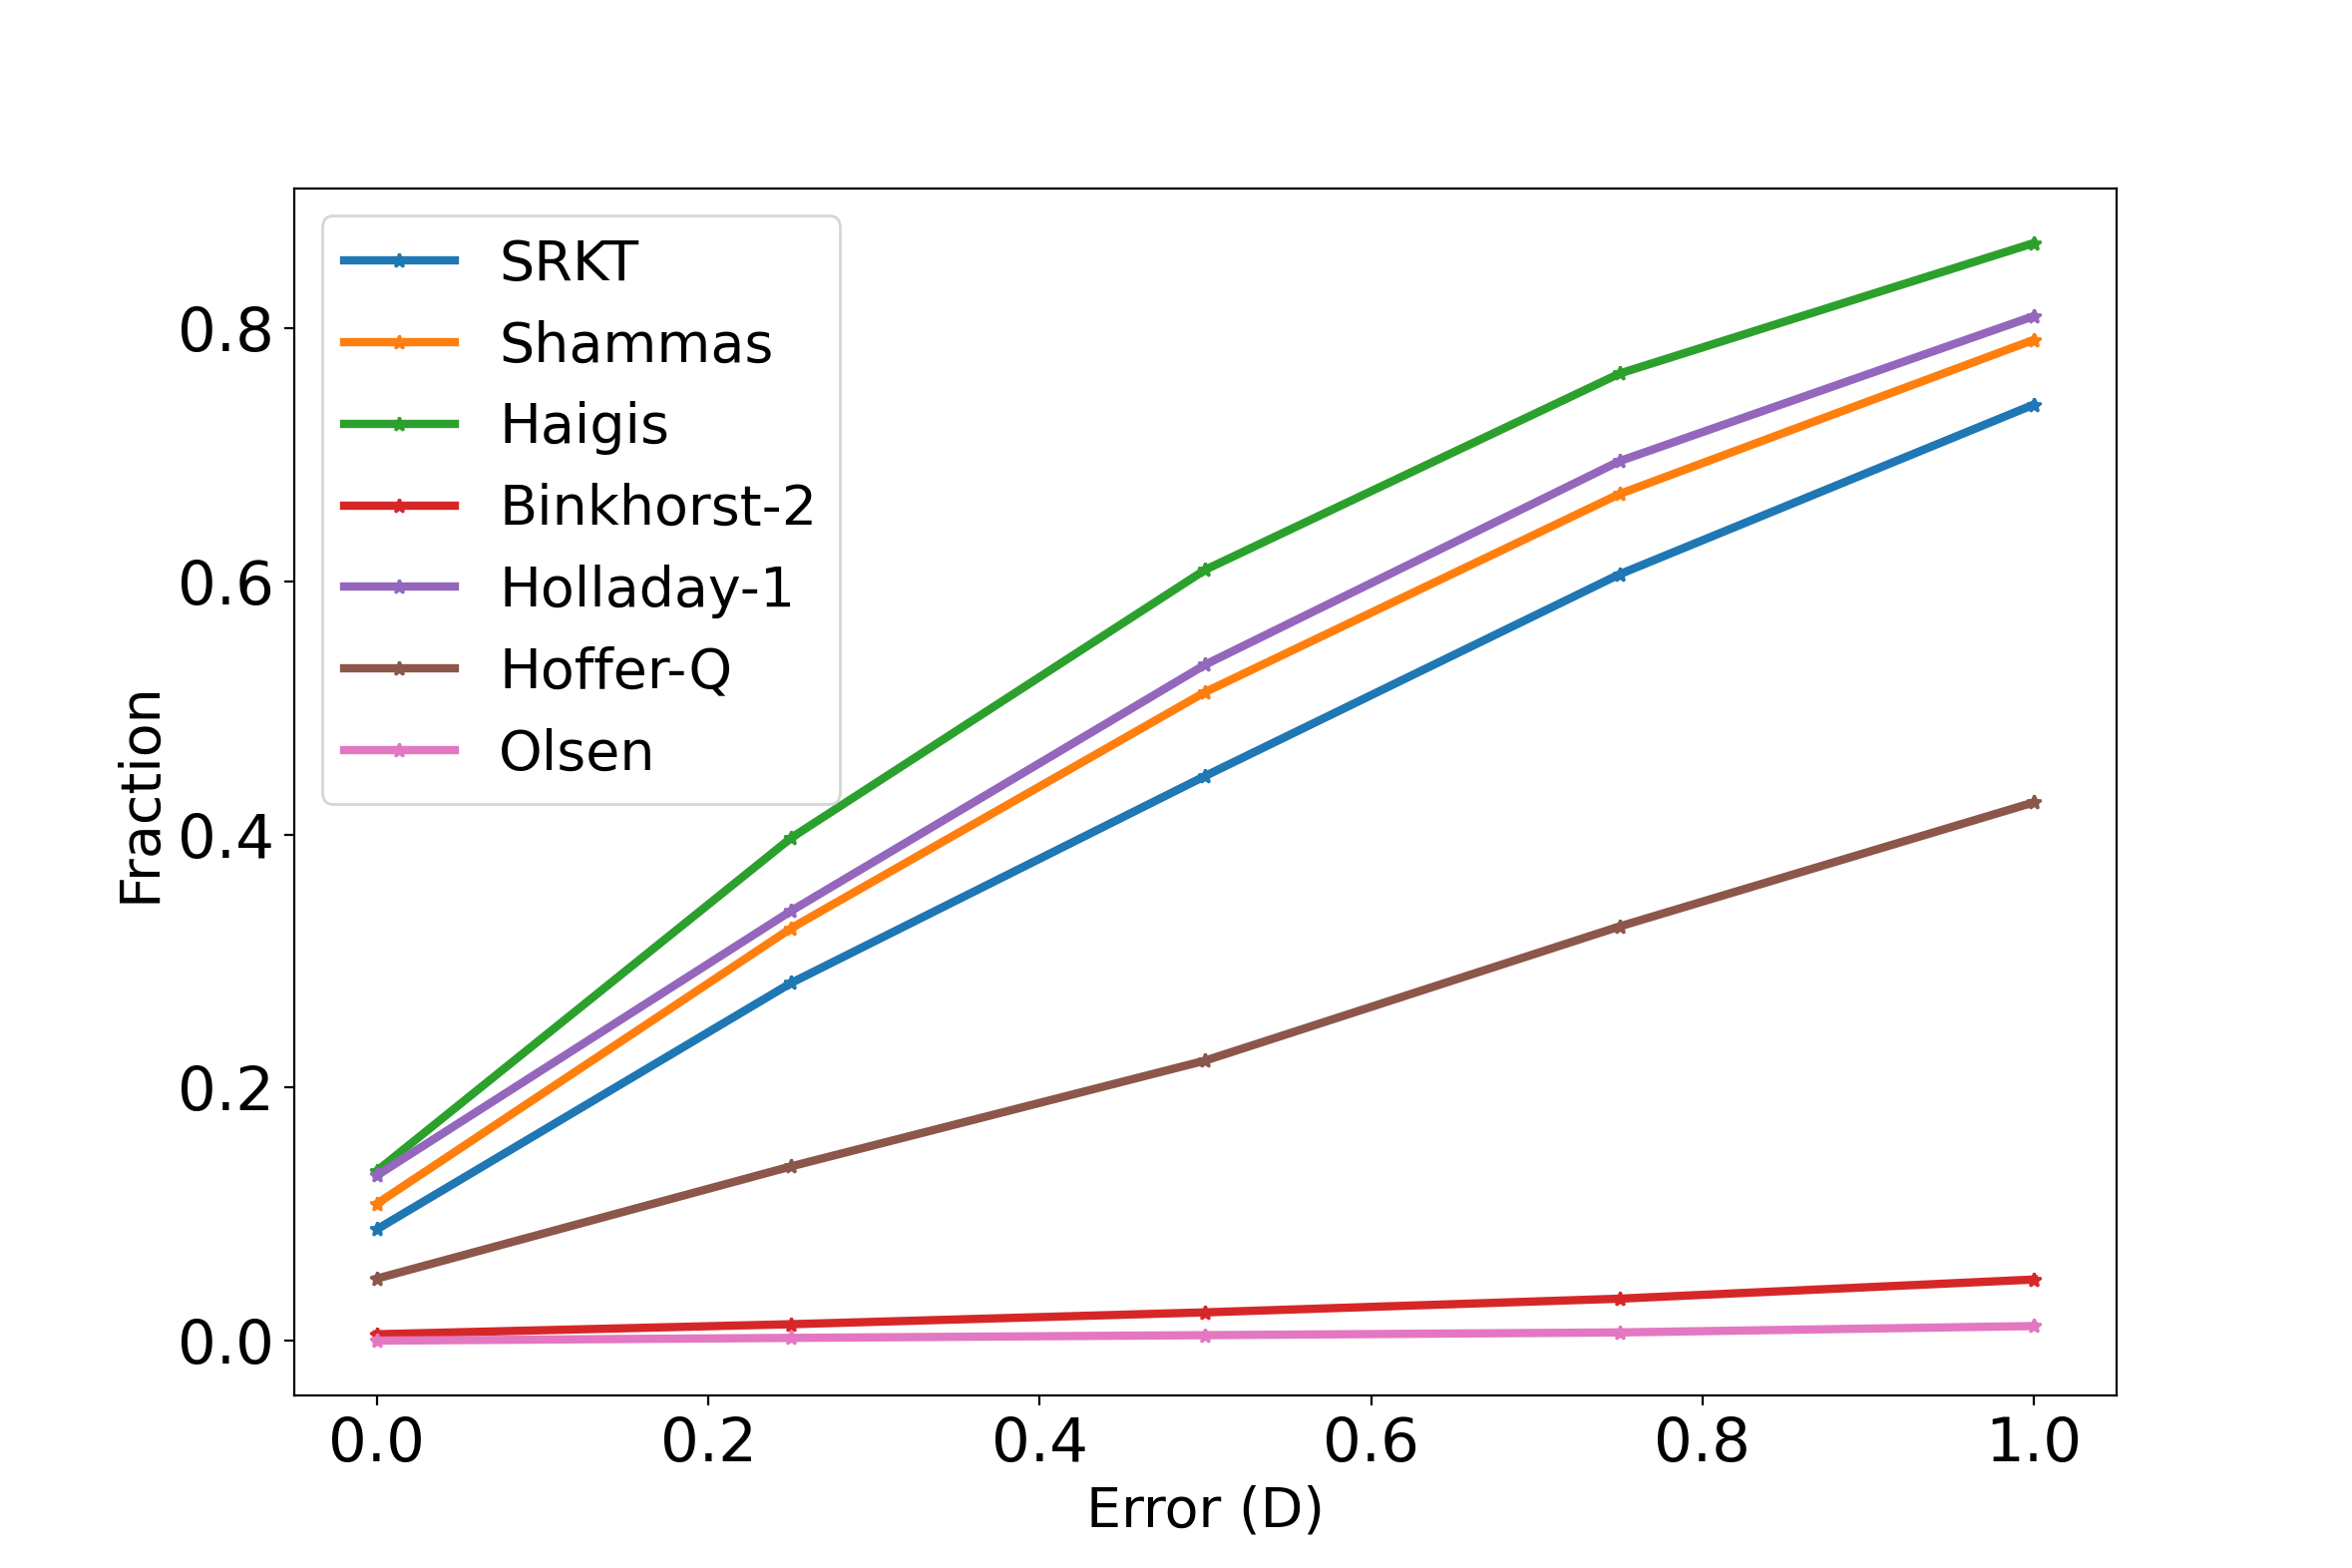
\includegraphics[width=1\linewidth]{cumulativeAbsoluteErrorFormulas_implantedPower}
	\caption{Cumulative absolute error $|R-R_f|$ of IOL formulas given the power implanted $P_i$.}
	\label{fig:cumulativeRefractionError_powerImplanted}
	\end{figure}

\subsection{Mean absolute refraction error}
To further benchmark formulas,  we compute the refraction MAE $|R-R_f|$, with the predicted $R$ (Eq. \ref{eq:expectedRefraction}, rounded to nearest quarter of diopter) vs.  the final post op visual acuity $R_f$.  We  found that the MAE from all formulas is 0.55D.  The cumulative refractive error was similar in all equations, with 26\% with no error, 47\% below 0.25D, 68\% below 0.5D, 85\% below 0.75D, and 91\% below 1D error from final refraction. In Fig. \ref{fig:histogramOfRefractionErrorFormulas} we present the distribution of the refraction error by all formulas in this study from final refraction after rounding the predicted power to nearest half diopter. Further rounding the predicted refraction to nearest quarter of diopter, results in no difference between the refraction error histograms of formulas (data not shown). This result shows that no apriori distinction between formulas can be made using the MAE.
\begin{figure} 
	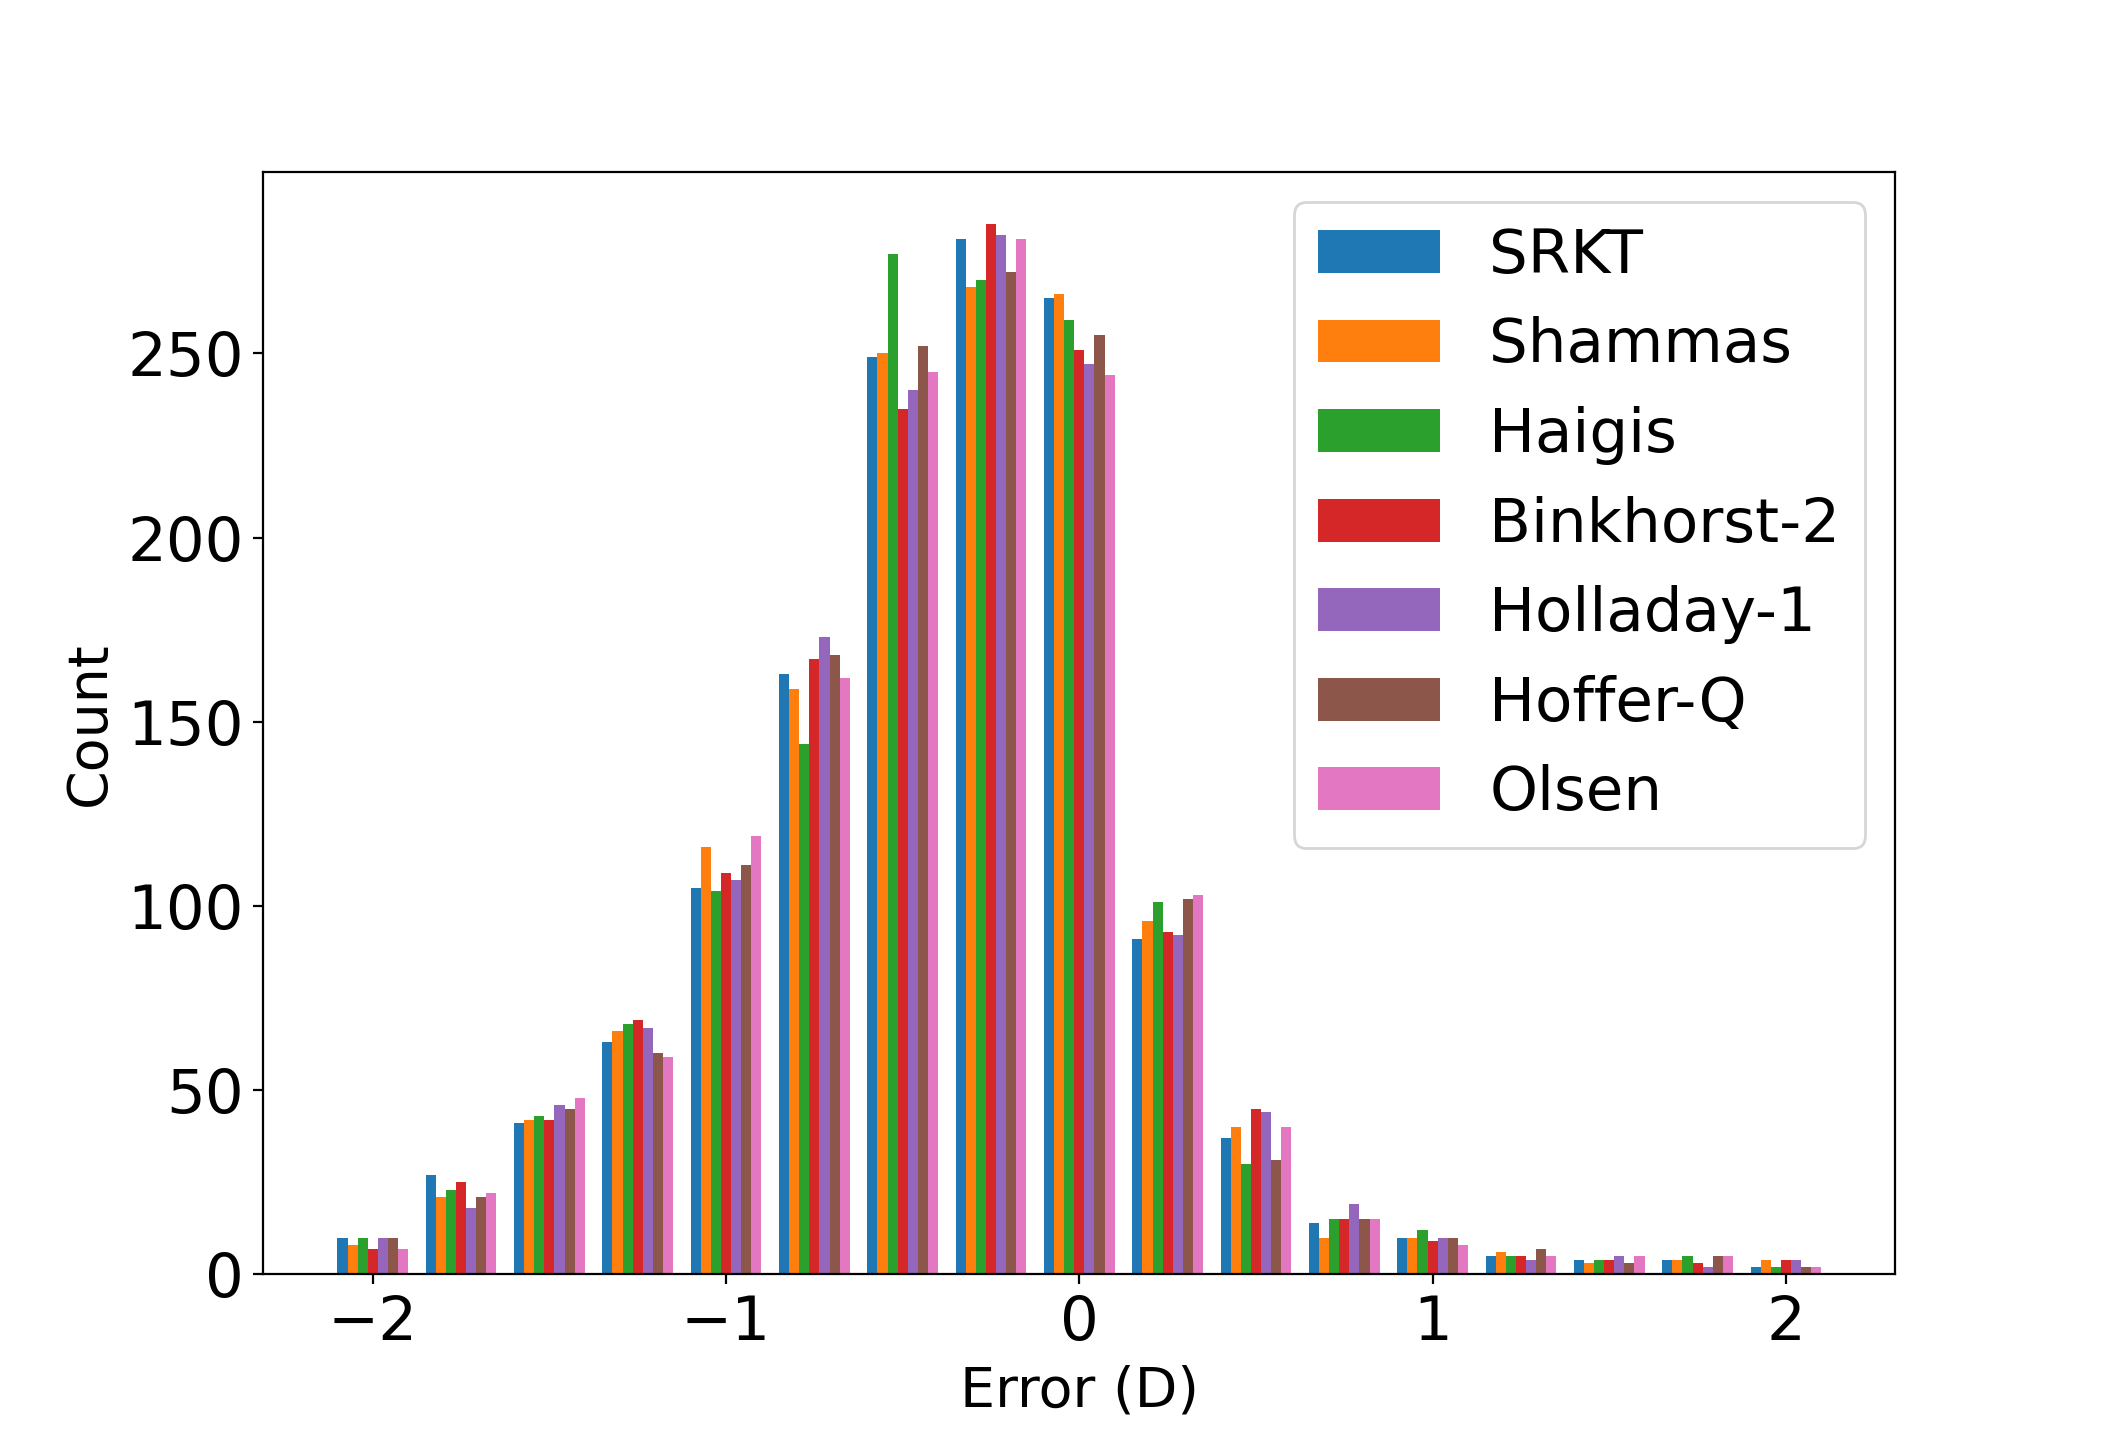
\includegraphics[width=1\linewidth]{Histogram_RefractionError_Formulas}
	\caption{Histogram of absolute refraction error $|R-R_f|$, with $R$ the predicted refraction after rounding the predicted power to nearest half diopter.}
	\label{fig:histogramOfRefractionErrorFormulas}
\end{figure}

\subsubsection{Regressors for $\Delta R$ perform equally between IOL formulas}
Next, we set out to predict the residual refraction post op. $\Delta R$, which will allow us to correct the suggested power from any formula, to arrive more closely to target refraction. To predict $\Delta R$, we trained and validated a linear regressor for each one of the 7  IOL formulas in this study, as described in Methods \ref{subsection:predictingRefractiveError}.
The training set included 1179 samples chosen uniformly at random, and we examine the accuracy of regressors using the reminder 208 samples in out dataset.
In Fig. \ref{fig:cumulativeErrorRegressors} we present the cumulative $\Delta R$ errors for the validation set. We find that for the trained regressors, all formulas achieved similar regression residual error $E_{reg}$ (Eq. \ref{eq:regressionCumError} with: 20\% of observations with no error, 60\% equal or below 0.25D, 80\% below or equal 0.5D, and 90\% below or equal 0.75D, which shows that predictions to the refraction errors $\Delta R$ can be made equally accurate for any formula. 
\begin{figure}
	\centering
	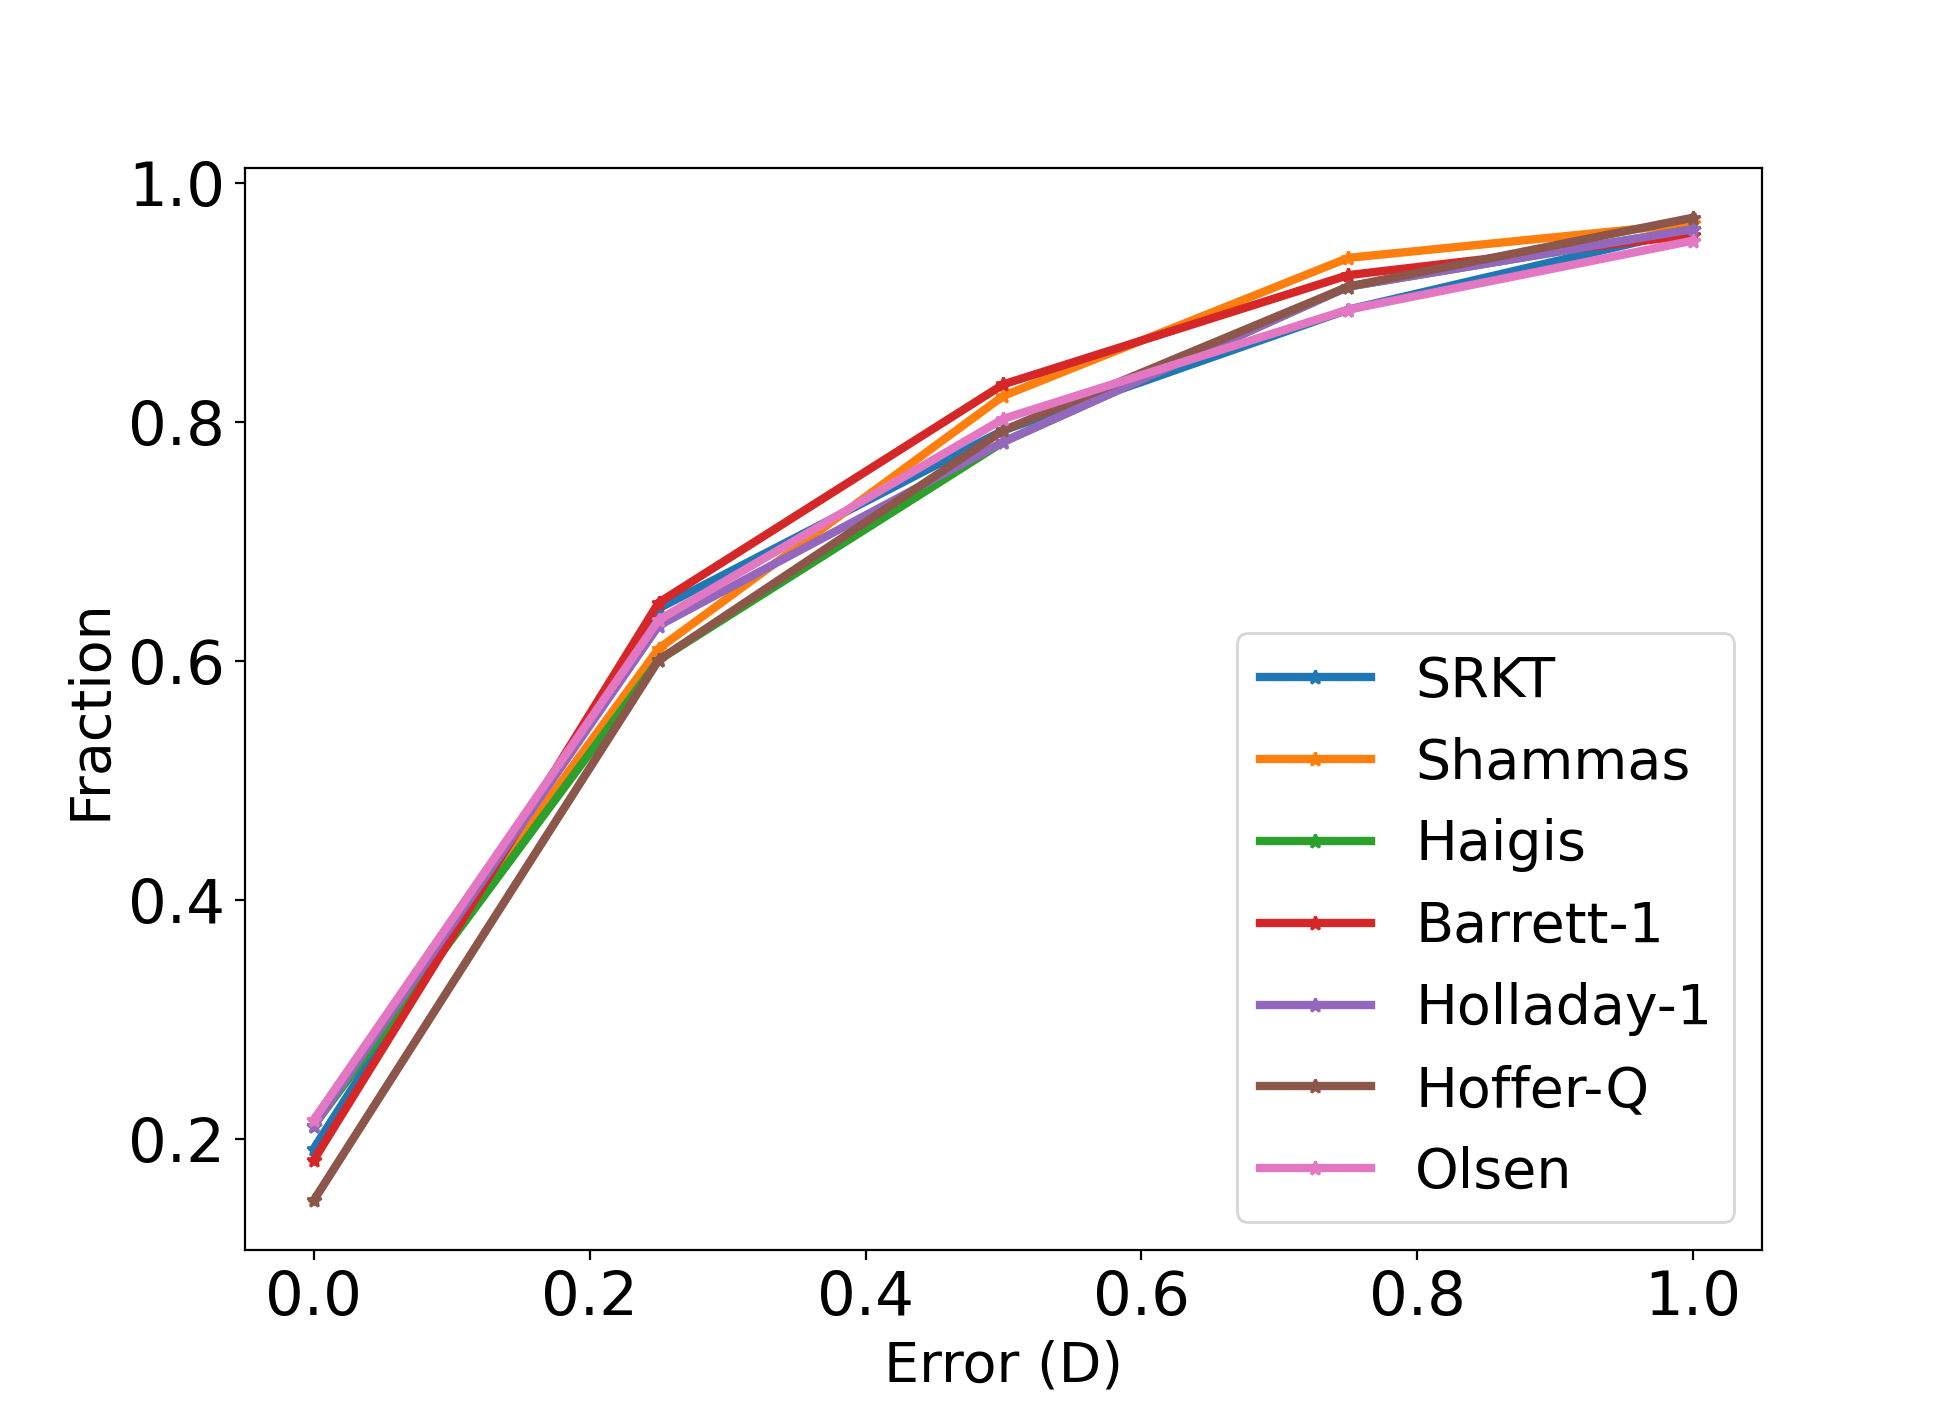
\includegraphics[width=1\linewidth]{cumulativeRefErrRegressors}
	\caption{Cumulative fraction of observations below a refraction error threshold 0, 0.25, 0.5, 0.75, and 1D, predicted by our trained regressors for each IOL formula in this study. The performance of all trained regressors is relatively similar on the validation set, with about 60\% of observation below 025D error, about 80\% below 0.5D and 90\% below 0.75D.}
	\label{fig:cumulativeErrorRegressors}
\end{figure}
We then compute the correction to the IOL power $\Delta P$ given predicted $\Delta R$. A summary of the computed $\Delta P$ and $\Delta R$ for training and validation set appear in Table \ref{table:refractionAndPowercorrectionResults}.
\begin{table}
	\begin{tabular}{l|c|c|c|c|}
		  &\multicolumn{2}{c}{Training} &\multicolumn{2}{c}{Validation}\\		  
		 &  $\langle \Delta R\rangle $ & $\langle \Delta P\rangle $  & $\langle \Delta R\rangle$ & $\langle\Delta P\rangle $ \\
		 \hline 
		 SRK/T         & 0.37 & -0.51 & 0.37   & -0.53\\
		 Shammas   & 0.38 & -0.50 & 0.39  & -0.51\\
		 Haigis        & 0.34 & -0.50 & 0.34  & -0.52\\
		 Binkhorst-2 &0.37 & -0.47 & 0.37  & -0.48\\
		 Holladay-1 & 0.38 & -0.57 & 0.38  & -0.58\\
		 Hoffer-Q   & 0.39 & -0.55 &  0.39 & -0.57\\
		 Olsen        & 0.38 & -0.45 &  0.38  & -0.45
	\end{tabular}
\caption{Mean refraction error $\langle \Delta R\rangle$ and mean computed power correction $\langle \Delta P\rangle$ predicted by our trained regressors for each one of the IOL formulas in this study, for the training (two left columns) and validation sets (last two columns).}
\label{table:refractionAndPowercorrectionResults}
\end{table}
We note that other regressors were trained and examined for their accuracy and despite achieving higher accuracy in the training set, the prediction on the validation set remained similar to the linear regressors. These regressors tended to over-fit the training set, but performed poorly on the validation and were thus excluded from further consideration. 
From Table \ref{table:refractionAndPowercorrectionResults}, we appreciate that the majority of regressors performs equally well in training as on the validation set, indicating their stability and repeatability. The mean refraction error $|\Delta R -\Delta R_o|$ for the validation set was -0.5D (rounded values).

Despite the equal average performance among regressor, we find that predicted refraction errors differ between observations, which indicate that the performance of different regressors is better on different regions of the parameter space (e.g. axial length, ACD, etc). The descrepency between regressors can be evaluated by the coefficients of the multi-linear regressors. Overall, These observations motivates the construction of a classifier to automatically select the most suited regressor given a set of objective measurements, to minimize $|\Delta R-\Delta R_o|$. 

\subsubsection{Automatic selection of IOL formula}\label{subsection:AutomaticSelectionOfIOLFormula}
Next, we set out to construct a predictor for the regressor (IOL formula) to be used based on patient-specific measurements. For this end, we trained a KNN classifier, after performed hyperparameter tuning using grid-search with cross validation (see Methods) on 85\% of our database (1179 observations). The optimal classifier parameters for our task appear in Table \ref{table:KNNparameters}.
\begin{table}
	\begin{tabular}{l|c}
		KNN parameter  & Value\\
		\hline 
		\hline 
		n neighbors & 5 \\
		algorithm  & kd tree\\
		leaf size   & 10 \\
		p    & 1\\
		weights & distance
	\end{tabular} 
  \caption{Values of the hyperparameters of the KNN classifier. Parameter names follow convention in python sklearn framework.}
  \label{table:KNNparameters}
\end{table}
Features used in classification are: pre-op. axial length $L$, the pre-op ACD, average keratometry, and target refraction $R_t$. Details of the classification process appear in Methods subsection \ref{subsection:ClassificationOfIOLFormulas}. 

We find that  our classifier correctly assigned labels (formula) is 85\% of cases. We note here that multiple classes which produce the minimal $\Delta R-\Delta R_o|$ were equally possible. Hence, we took that into consideration when computing the accuracy of our classifier. 
After classification on the validation set, we use the chosen regressors (classes) for each set of objective measurements to predict the $\Delta R$ and then substituted it in Eq. \ref{eq:expectedPower} to compute the IOL power correction $\Delta P$. 
In Fig. \ref{fig:HistogramOfChosenFormulas} we display a histogram of the predicted formulas from  the validation set.
\begin{figure}
	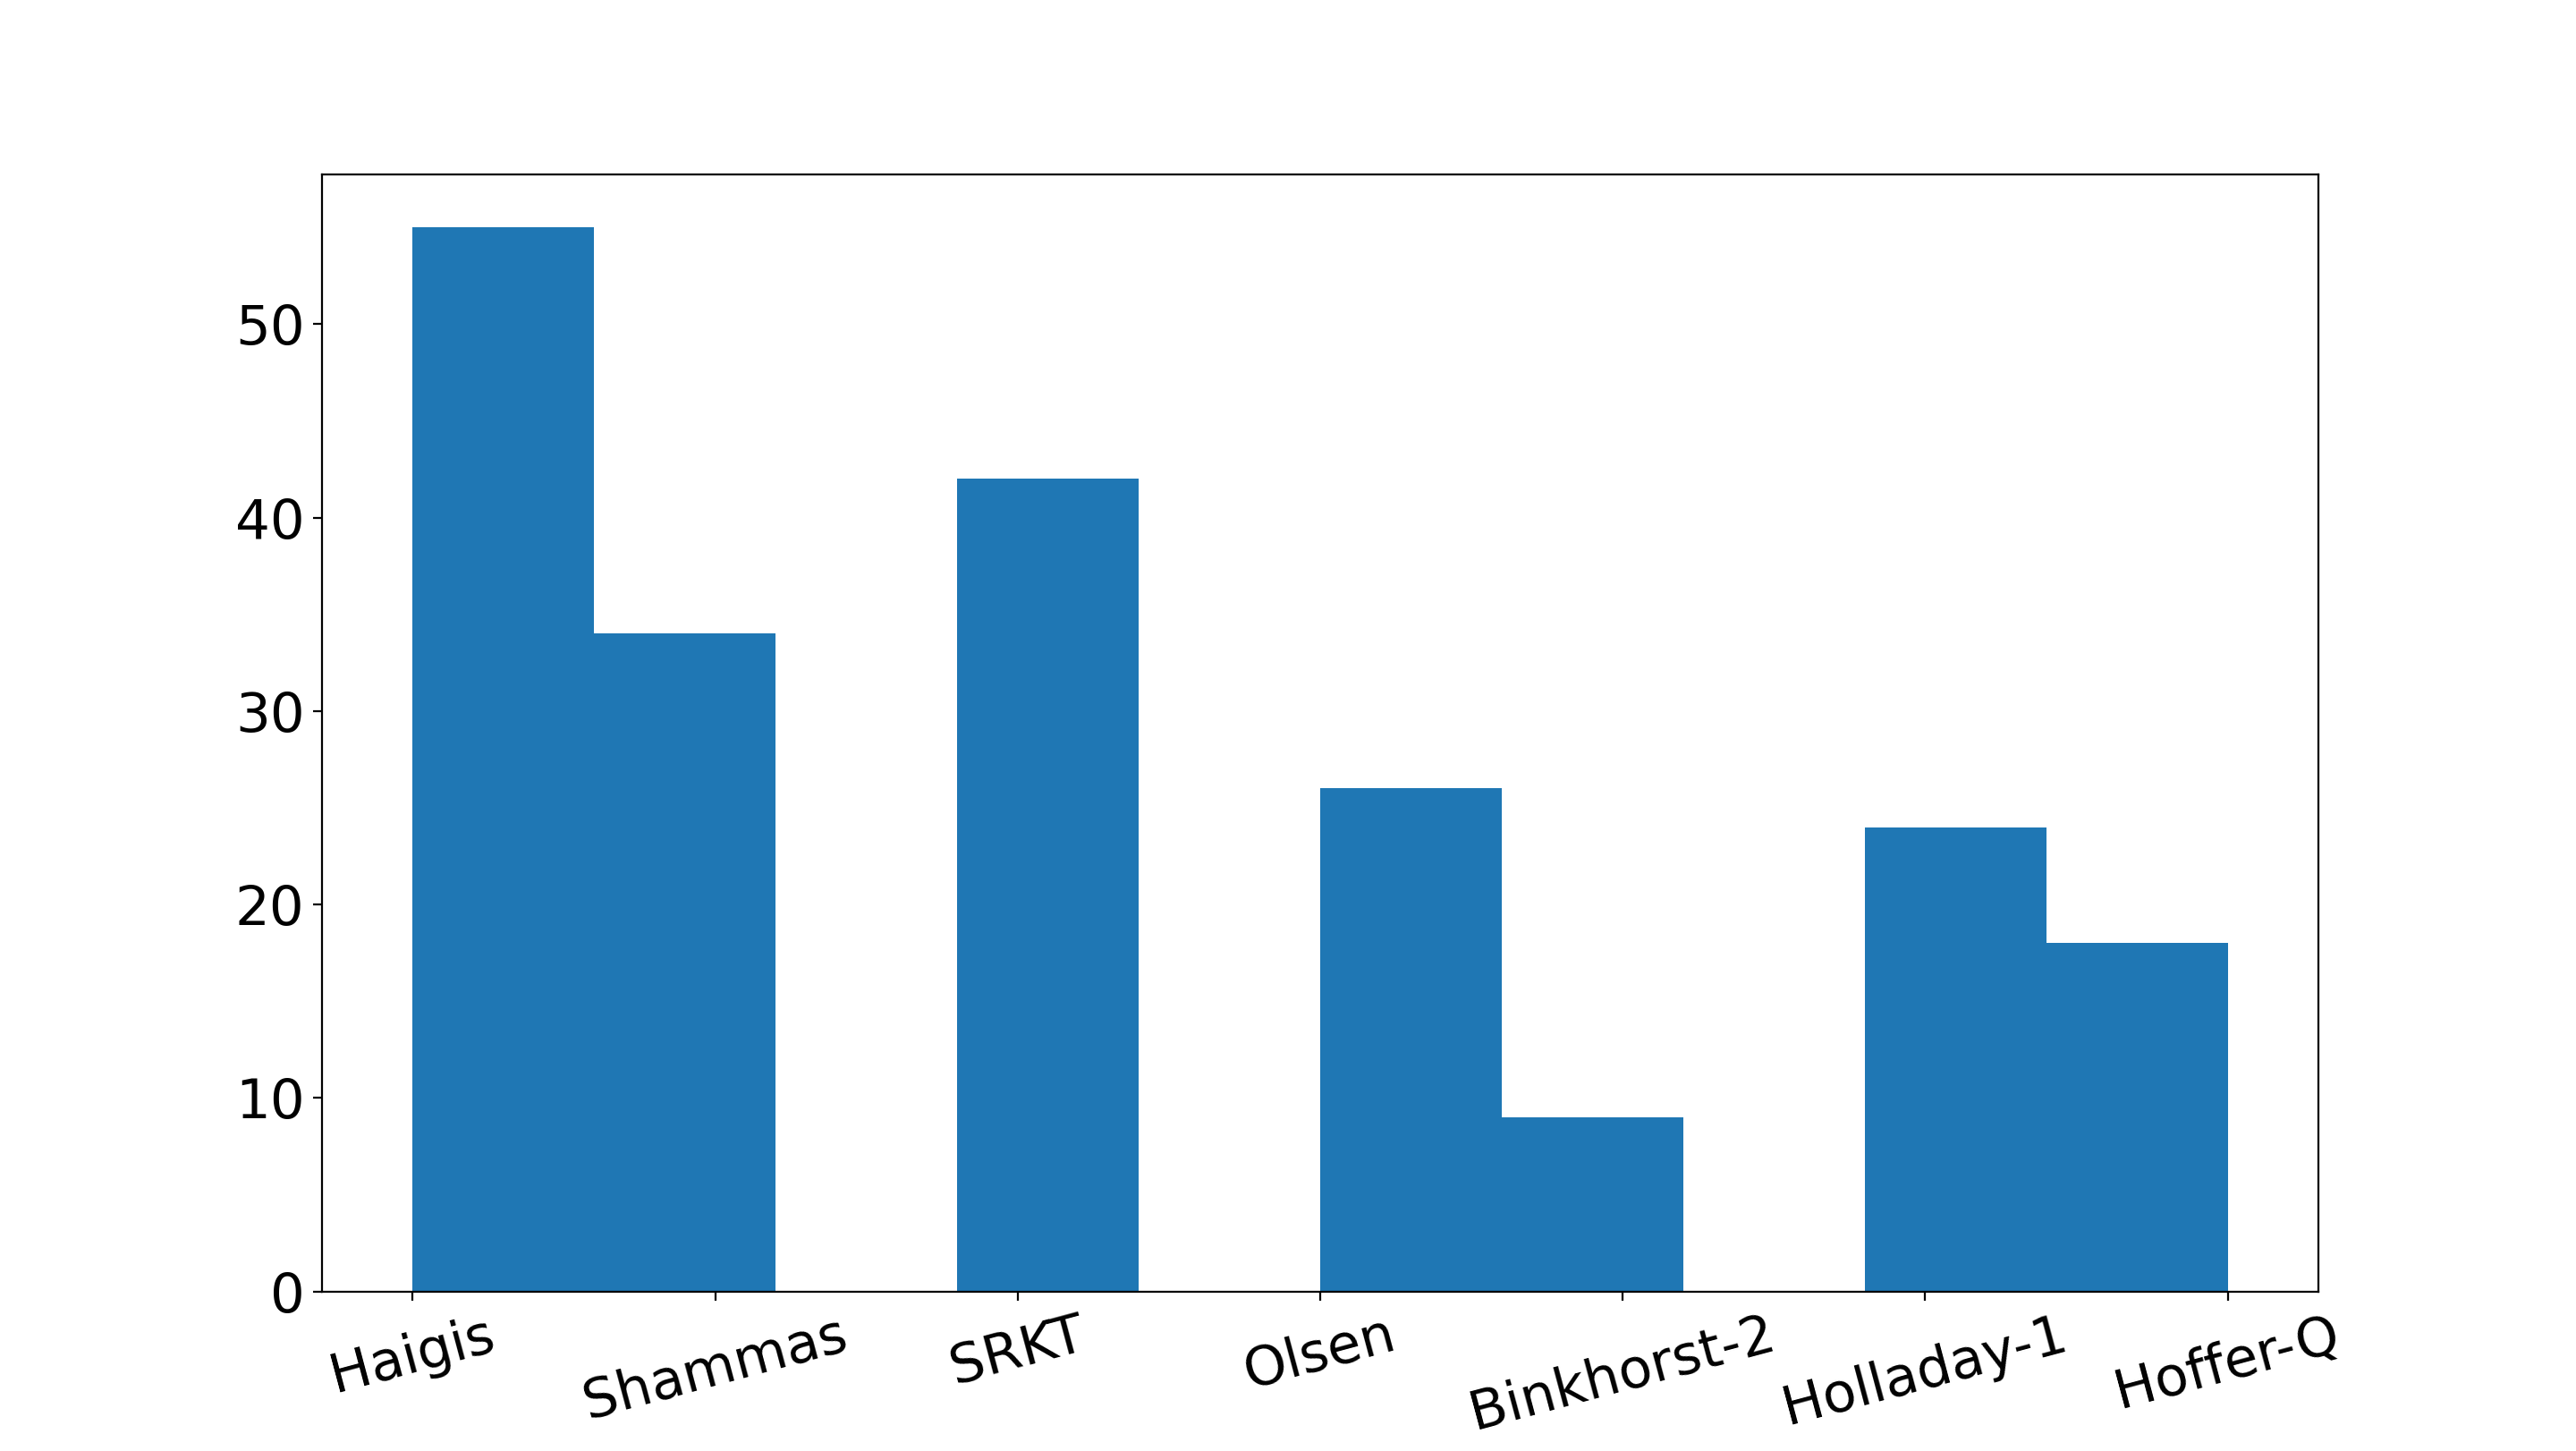
\includegraphics[width=1.1\linewidth]{HistogramOfChosenformulaAfterClassification}
	\caption{Histogram of IOL formulas resulting from automatic classification by our model.}
	\label{fig:HistogramOfChosenFormulas}
\end{figure}
The  theoretical minimum $\Delta R-\Delta R_o$ was 0.33D, which would have resulted from a perfect classification, whereas we obtain $\Delta R-\Delta R_o|=0.35D$ after classification. 
In Fig. \ref{fig:cumulativeddRFormulaVsPredicted} we plot the cumulative absolute difference  $|\Delta R - \Delta R_o|$ after classification vs. the refraction error $\Delta R$ from individual formulas, showing that after classification we can obtain lower predicted refraction error.
The mean predicted $\Delta R-\Delta R_o$ was 0.3D, resulting in a mean predicted $\Delta P$ of -0.47D, which is the IOL power correction needed to arrive at target refraction. 

\begin{figure}
	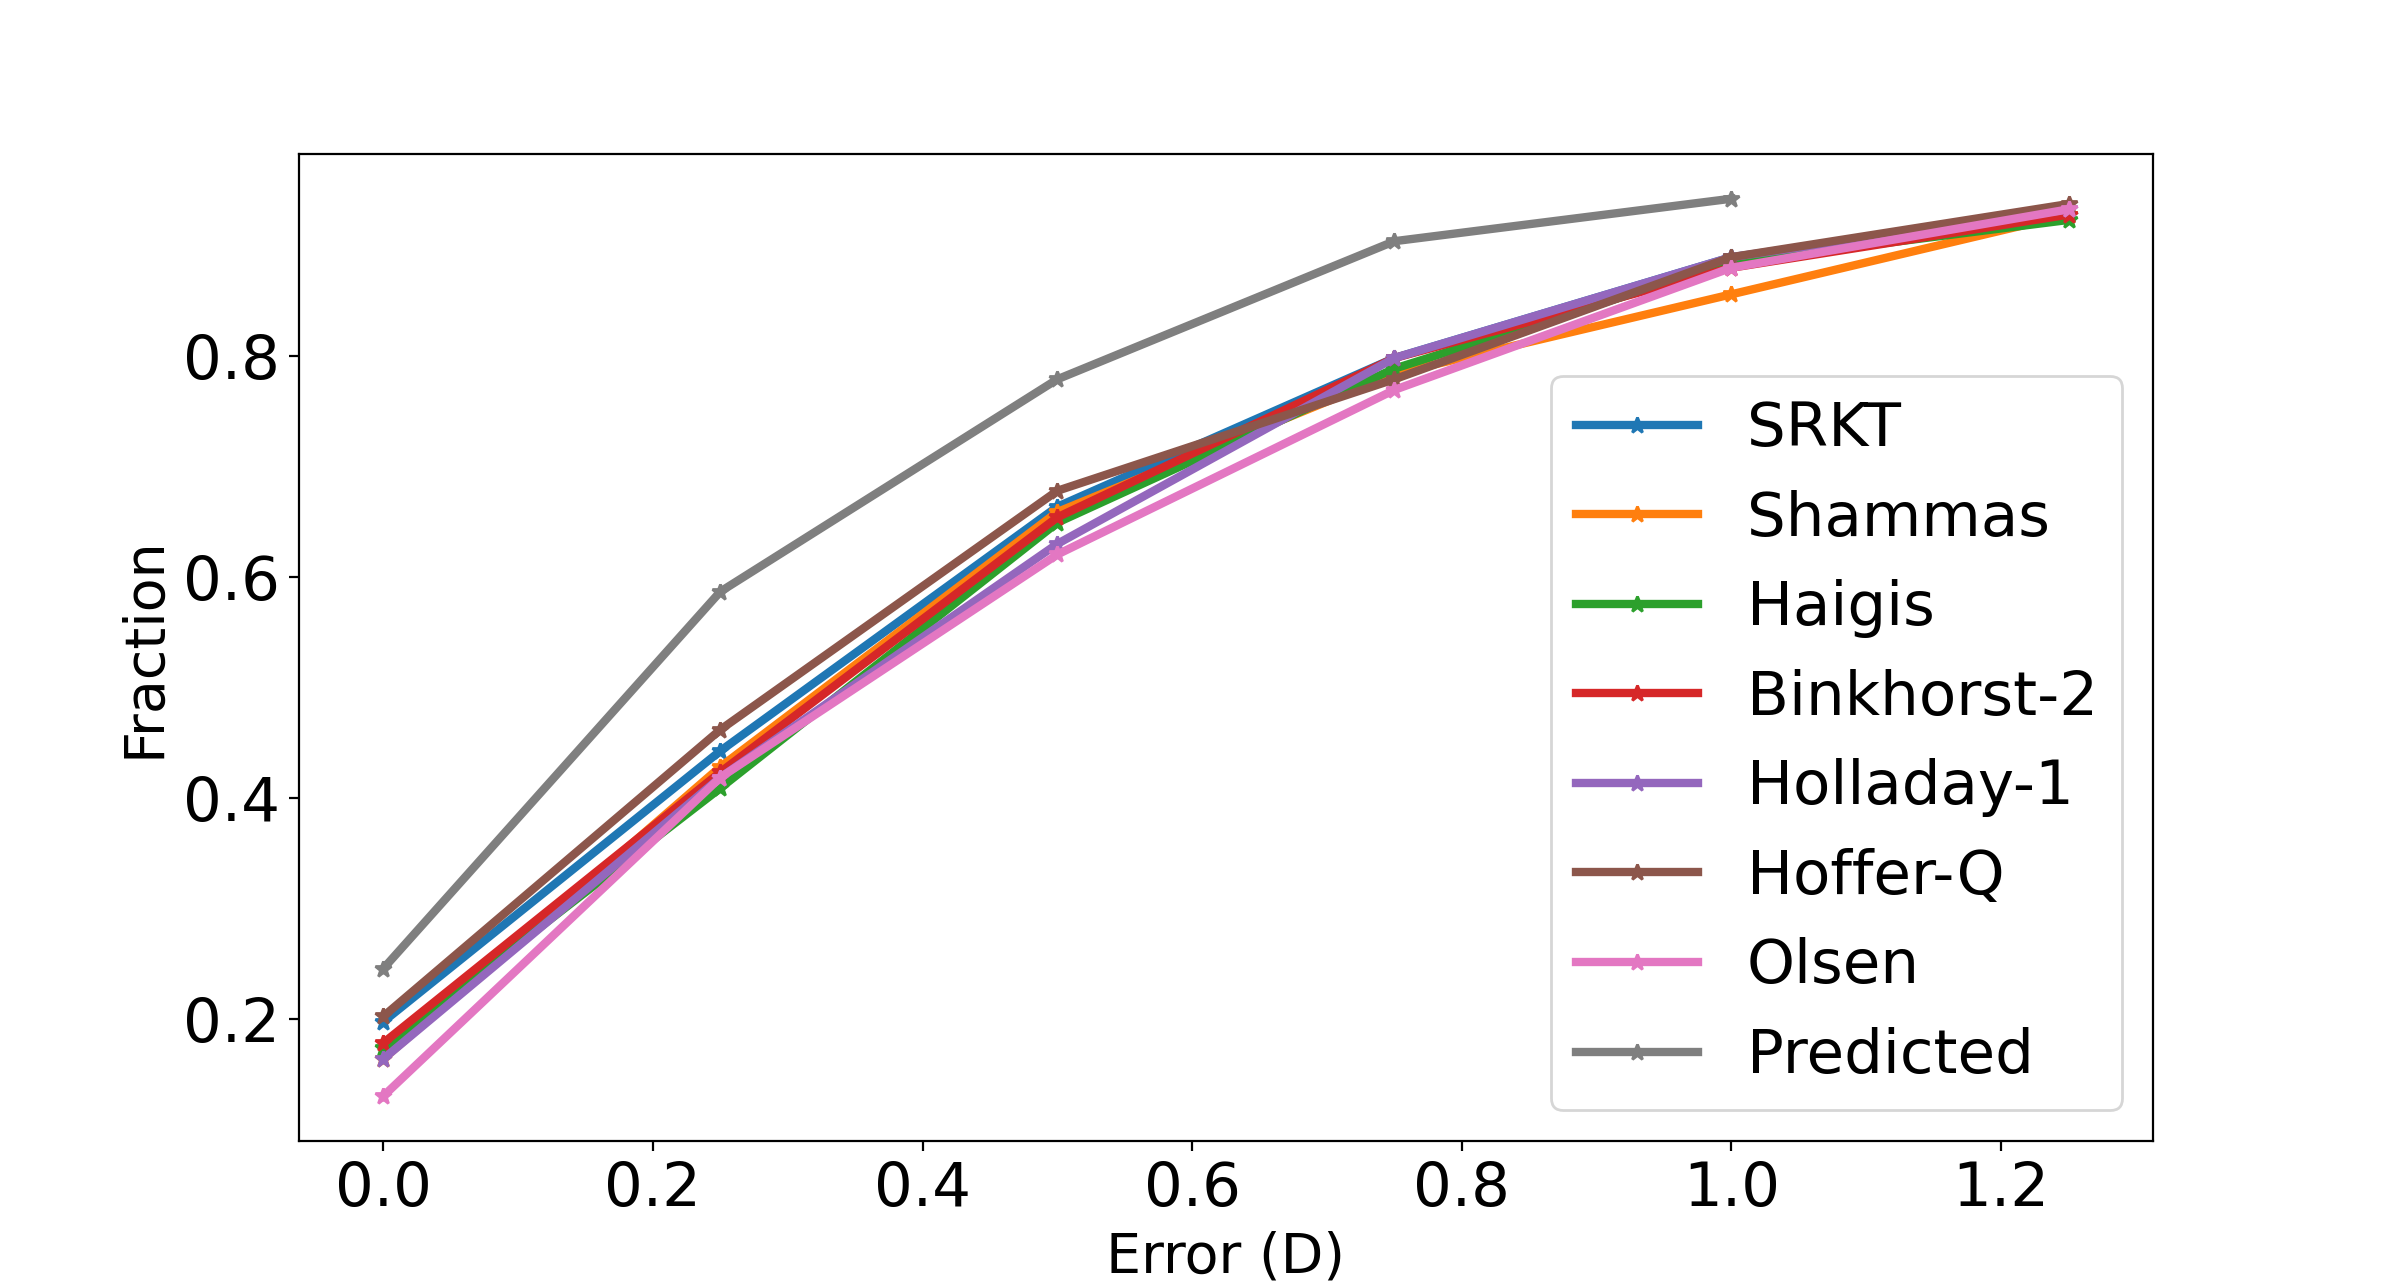
\includegraphics[width=1\linewidth]{dRFormulasVsClassification.png}
	\caption{Cumulative refraction error of prediction $|\Delta R-\Delta R_o|$ (gray) vs refraction error $\Delta R=|R-R_f|$ from individual formulas.}
	\label{fig:cumulativeddRFormulaVsPredicted}
\end{figure} 

 %in Figure \ref{fig:RefErrVsAxialLengthAlpha1} for $alpha=1$, with the refraction error shown without the absolute value to emphasize the spread of the refraction error of our algorithm around zero vs. other IOL formulas. 
%\begin{figure}
%	\centering
%	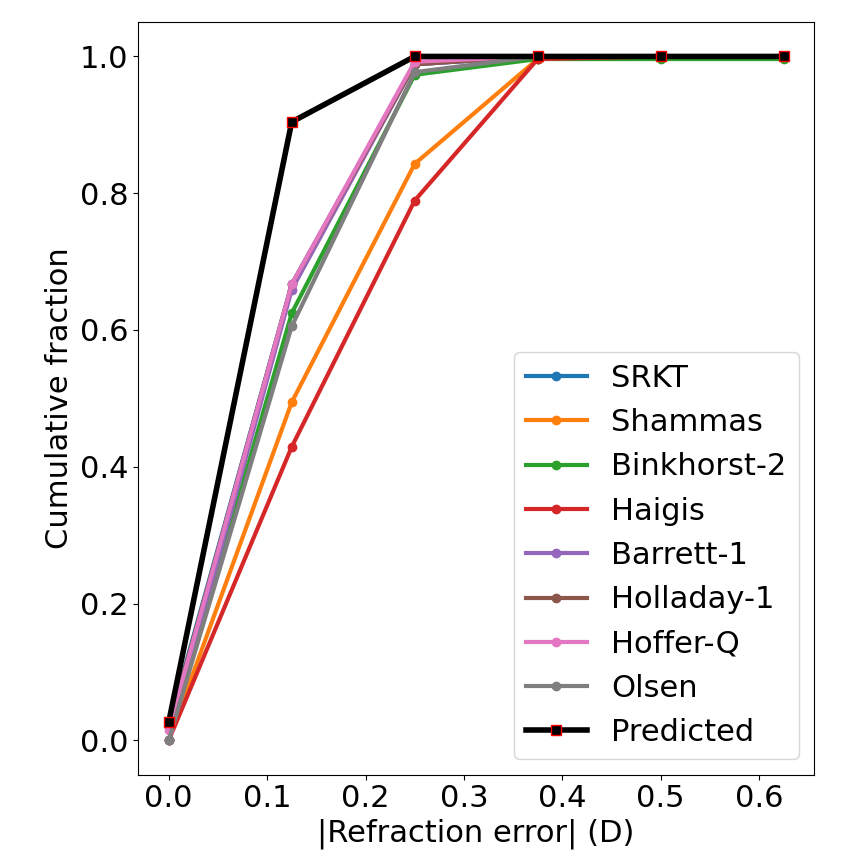
\includegraphics[width=1\linewidth]{cumulativeRefErrAlpha1}
%	\caption{Cumulative percentage of observations below an absolute refraction error $|R_f-R|$ in intervals of 0.125D, shows our prediction method (black) is superior to the 8 IOL formulas tested, with 92\% of observations below 0.125D error using our prediction method.}
%	\label{fig:cumulativereferralpha1}
%\end{figure}


%In Figure \ref{fig:RefErrVsAxialLengthAlpha1} we plot the refraction error $|R_f-R|$ as a function of the axial length, showing that our predictions (red circle) are all within the range $\pm0.125D$.
%\begin{figure*}
%	\centering
%	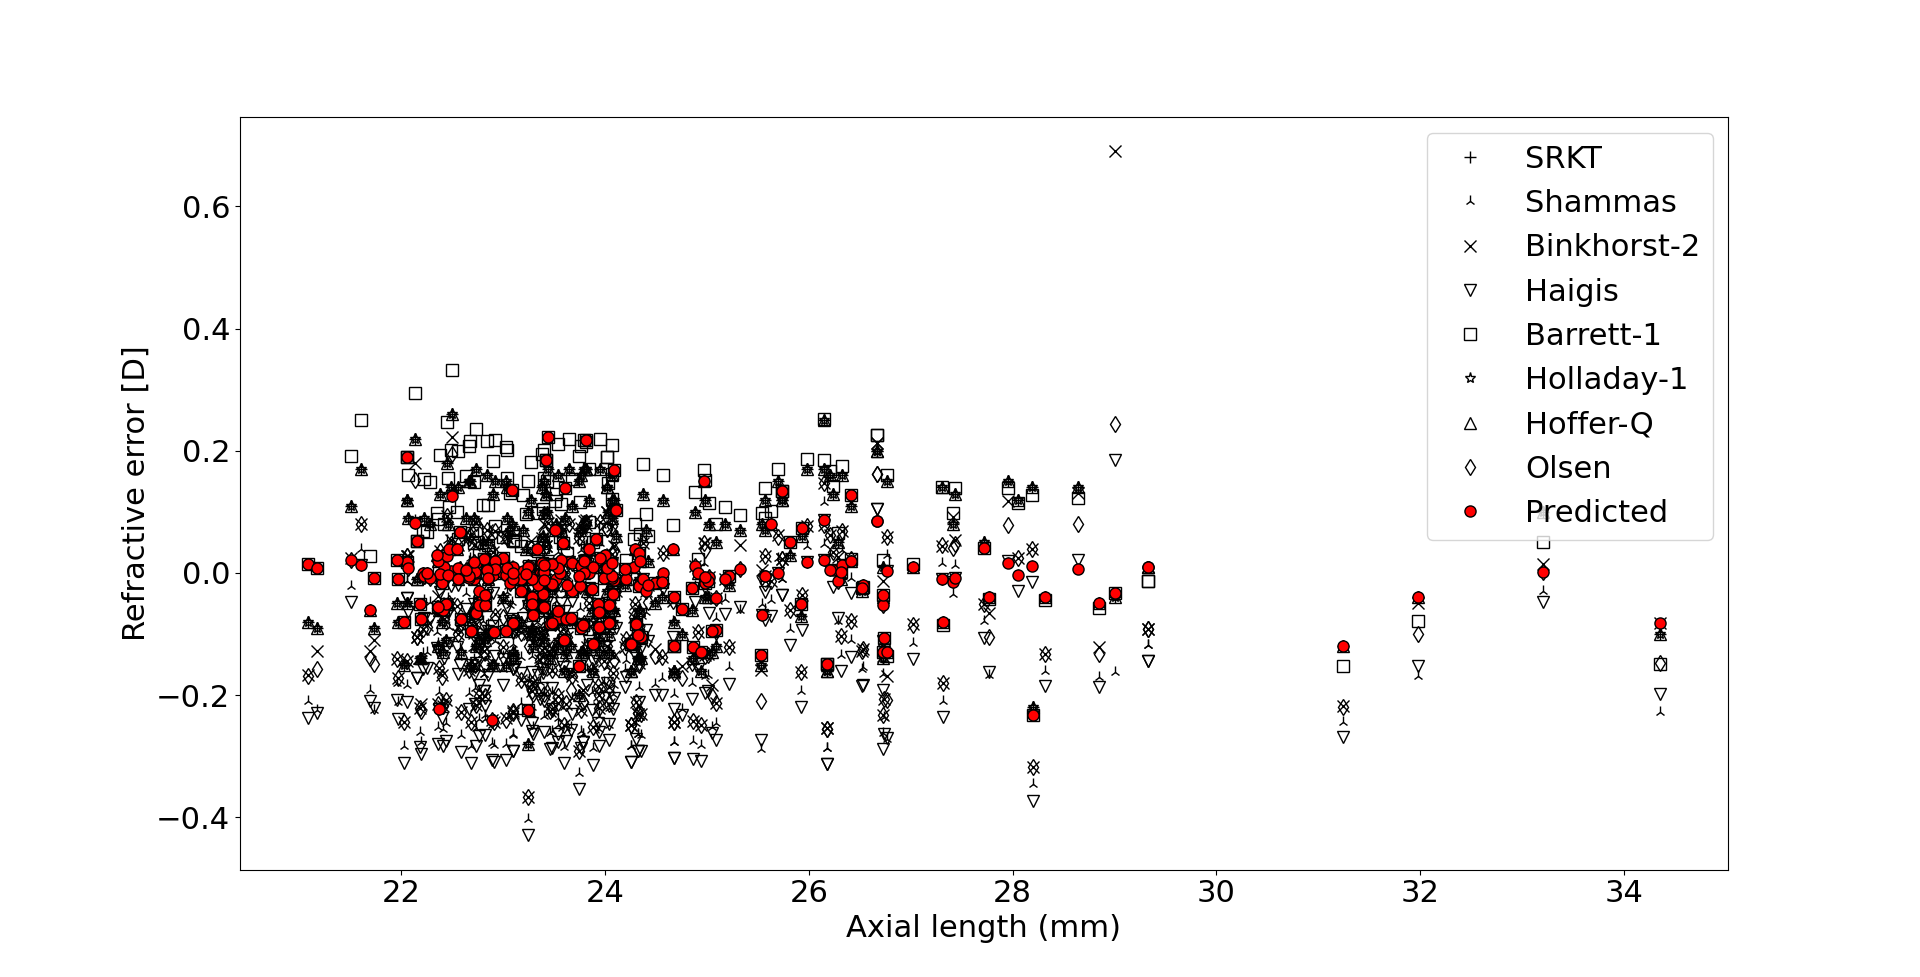
\includegraphics[width=1\linewidth]{RefErrVsAxialLength_alpha1}
%	\caption{Refraction error $R_f-R$ as a function of the axial length. Our predictions in red circles, showing a consistent refraction error in the range of $\pm0.125D$ for all values of the axial length.}
%	\label{fig:RefErrVsAxialLengthAlpha1}
%\end{figure*}

%\begin{figure*}
%	\centering
%	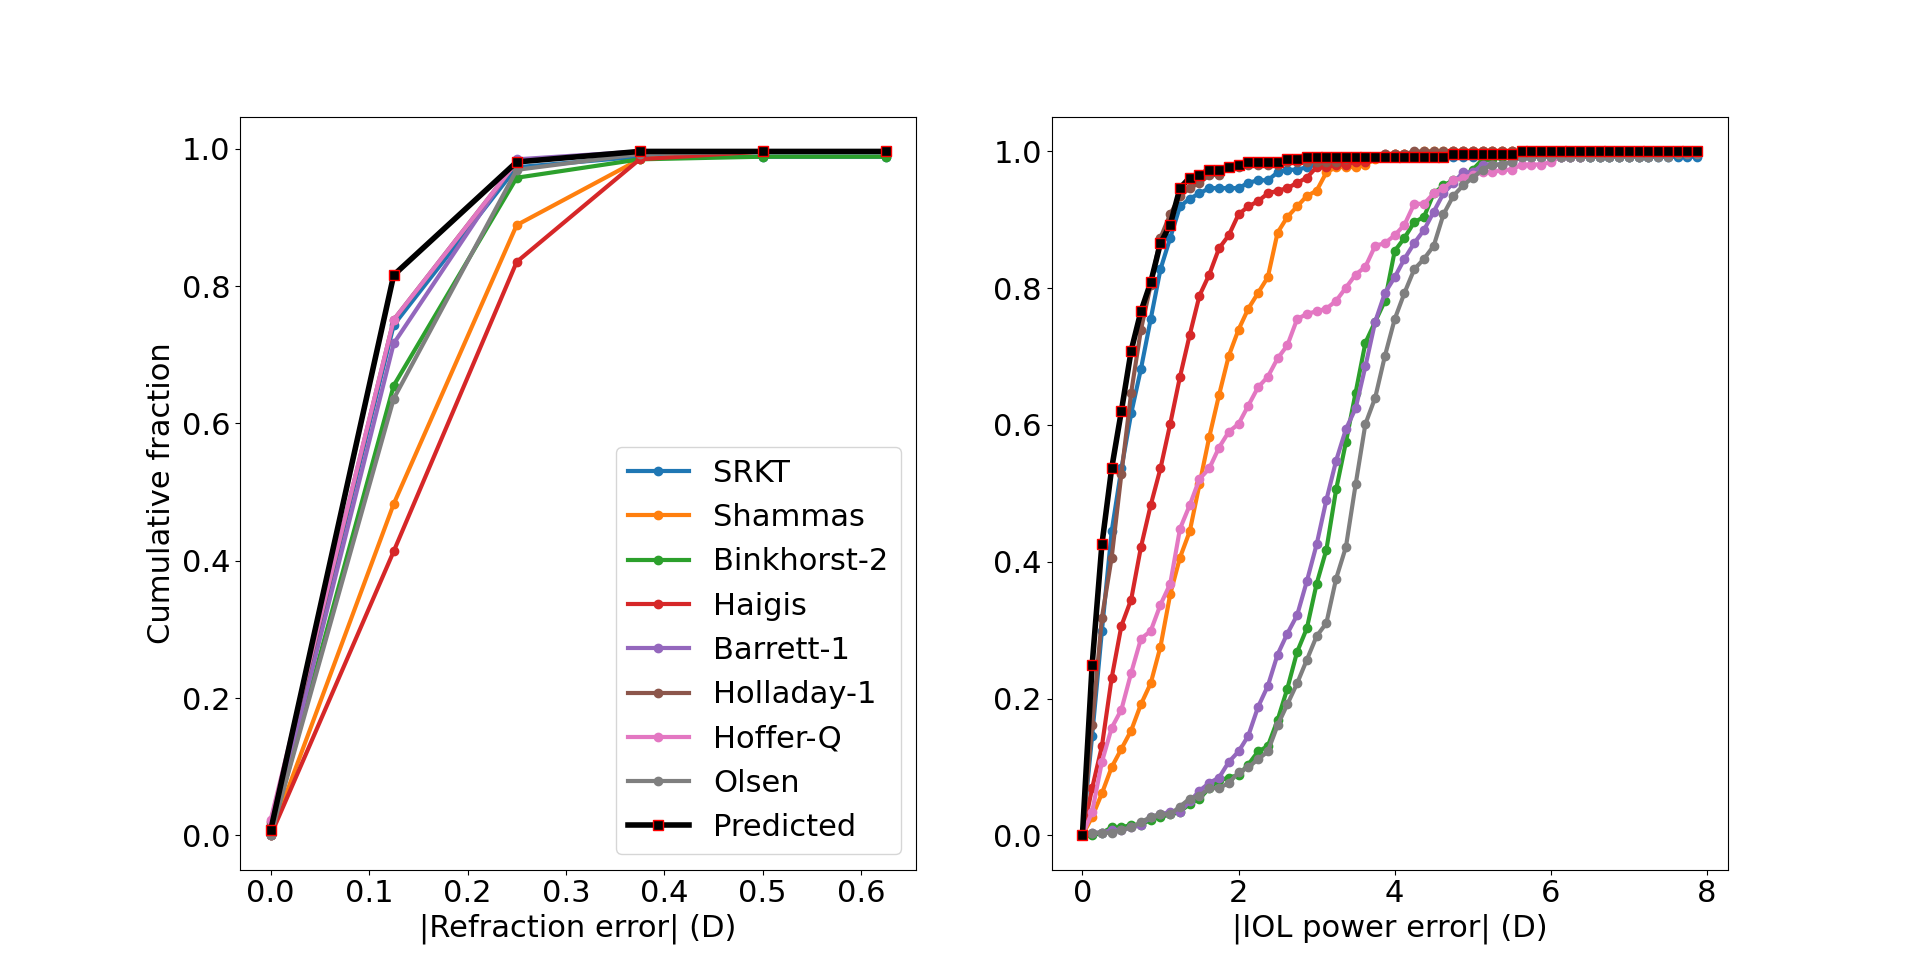
\includegraphics[width=1\linewidth]{powerAndRefErr_alpha0_6}
%	\caption{Cumulative fraction of observations below a certain refraction error (left panel) and below certain power error (right panel). Our prediction method appears in black. using our prediction methods for $\alpha=0.6$, 82\% of predictions fall below refraction error of 0.125D and }
%	\label{fig:PowerAndRefErrAlpha06}
%\end{figure*}

\section{Discussion}\label{section:Discussion}
In this work we have presented a combined regression-machine learning framework to correct the IOL power predicted from IOL formula, thus to arrive more closely to target refraction. Our work is motivated by the observation that physician tend to manually correct the IOL power suggested from a given formula, by using empirical rules of thumb. Indeed, we find that an average of 0.5D is subtracted from the IOL power predicted to arrive at the power finally implanted. Despite IOL power adjustment, residual post op refraction error remains, with and average of 0.4D. Here we devised a method to predict the residual refraction error, and then use the predicted value to compute the needed correction to the IOL power (Methods \ref{subsection:predictingRefractiveError} ). 
Indeed,  after training of regressors we found that an average of 0.5D needs to be subtracted, in line with what is observed in practice. This results thus shows that a physician can now be free of applying empirical rules of thumb to correct the IOL power at the surgery planing stage. 

A hierarchy between formulas in terms of the MAE is not a reliable scale. Indeed, we found that the MAE between power predicted and target refraction leads to a constant 0.55D absolute difference in all formulas. However, a hierarchy can still be created when using the power implanted to reverse compute the expected refraction. Doing so, still showed that the difference between formulas in terms of the MAE is not large enough to promote a given formula over others. In addition, a bias in such calculation exist, as the power implanted is derived from the equation used in the surgery planing stage. Had different formula was used in such planing, a different power to implant might have been finally used.
Our proposed framework, therefore, resolves the problem of forming a hierarchy between formulas  using the MAE, and instead automatically chooses the  predictor for the smallest $\Delta R-\Delta R_o$, which later results in the correction of IOL power needed to arrive at target refraction. 
In addition, various formulas operate differently in different regions of the parameter space (long or short eyes), our provides means of automatic selection of the formula without introducing rules of thumb and fudge factors. 

Our classifier achieved 85\% accuracy in classification IOL formula. Our methodology can be used without the IOL formula classifier and instead only correct for the IOL power of a given formula using the appropriate regressor. Indeed, we observe that the cumulative refraction error after classification does not differ much than that of each classifier alone (i.e 25\% at zero error, 60\% under 0.25D, 85\% under 0.5D and 90\% under 0.75D). However, The overall performance after classification was improved over that of each regressor separately. 

Clinical validation of the suggested method is not straightforward. Surgeons wil need to put confidence in the predicted $\Delta P$ from our algorithm, and then test the resulting VA post op. The resulting $\Delta R$ needs then to be compared to the observed $\Delta R $ in retrospective databases such as the one we used presently. 
In addition, a consistent recording of the ACD and axial length post op will greatly aid in estimating the accuracy of IOL formulas. These two variables can be used to assess the accuracy of each formula in predicting biophysical parameters, and thus serve as means of ranking formulas, in addition to the MAE currently used in practice. 

In summary, we presented here a framework for predicting the correction of the IOL power based on objective measurements from the IOL master. This framework is easy to implement in practice. Improvement to the current results can still be made, by exploring other regressor types instead of the linear regresors presented here, and further improve formula selection by replacing the KNN classifier by a more flexible methodology.


\section{Appendix}\label{section:iolFormulas}
\subsection{Deriving the relationship between $\Delta P$ and $\Delta R$}\label{subsection:derivationOfdPTodR}
We start with the Gaussian optics equation, and derive a relationship between the difference of two powers in terms of the difference in expected refraction. 
Let $L,e, K,$ be fixed for a given IOL formulas, and let the IOL power $P_1\neq P_2$ such that 
\beq
P_1 &=& \frac{n_v}{L-e}-\frac{n_c}{\frac{n_c}{K+R_1}-e}\\
P_2 &=& \frac{n_v}{L-e}-\frac{n_c}{\frac{n_c}{K+R_2}-e}
\eeq 
then 
$\Delta P = P_1-P_2$ is 
\beq 
\Delta P &=& n_c\left( \frac{1}{\frac{n_c}{K+R_2}-e}- \frac{1}{\frac{n_c}{K+R_1}-e}\right)\nonumber\\
 &=& n_c^2 \left(\frac{\frac{1}{K+R_1}-\frac{1}{K+R_2}}{ \left(\frac{n_c}{K+R_2}-e\right)\left(\frac{n_c}{K+R_1}-e\right) )}\right)\nonumber\\
  &=& n_c^2\left(\frac{R_2-R_1}{(n_c-e(K+R_1))(n_c-e(K+R_2))} \right)\nonumber \\
  &=&  \frac{-n_c^2\Delta R}{(n_c-eK-eR_t)(n_c-eK-e(R_t+\Delta R))} \nonumber \\
  &=& \frac{-n_c^2\Delta R}{\alpha^2 -e\alpha \Delta R} \label{eq:deriveddPtodR}
\eeq 
where here we set $R_1=R_t$ the target refraction, and $R_2=R_t+\Delta R$.
and 
\beq 
\alpha &=& n_c-e(K+R_t)\nonumber \\
\eeq 
The correction to the power predicted $P_1$ to reach target refraction $R_1=R_t$ is then $P_1+\Delta P$. 

%\subsection{Parameters of the trained classifier}\label{subsection:parametersOfClassifier}
%Parameters used for the RF classifier are summarized in Table \ref{table:parametersOfTheRFclassifier}. We examined a range of the hyper-parameters and found the listed ones a good compromise between size of the forest and the risk of over fitting the training data. The parameter names appears as in the sklearn package in Python.
%\begin{table}
%	\begin{tabular}{l|c}
%		Parameter     & Value \\
%		\hline 
%		\hline
%		n estimators  & 70 \\
%		criterion     & entropy \\
%		max. depth    & 150 \\
%		ccp alpha     & 1e-6\\
%		max. features & 3
%	\end{tabular}
%\label{table:parametersOfTheRFclassifier}
%\caption{The random forest classifier parameters used for training. Parameter names appearing here match the nomenclature of the sklearn Python package.}
%\end{table}
\subsection{IOL formulas}
Below, we summarize the calculation steps required for implementing several IOL formulas used in this research. The steps outlined in the next few subsections might differ in some parts from steps in the original publications of the methods. These modifications were made due to the presence of printing errors appearing in the original publications, which are corrected here.

\subsection{SRK}\label{subsection:srk}
The SRK IOL power calculation method is performed using the empirical regression formula
\beq
P = Aconst-0.9*\bar{K}-2.5*L,
\eeq 
with $P$ the IOL power (D), Aconst- the IOL manufecturer A-constant, $\bar{K}$ mean keratometry (D), and $L$ the axial length (mm).

To compute the resulting refraction 
\beq
R = P-1.5R_t,
\eeq 
with $R_t$ the target refraction (D)
The A-constant should be adjusted using retrospective data as follows:


\subsection{SRK/T}\label{subsection:srkt}
Set the refractive index $n_c=1.3375$. Start with a retrospective data computation of the individualized (surgeon) A-constant, or the $A_{indiv}$
\begin{enumerate}
	\item Use implanted power $P$, mean keratometry $K = 337.5/R_c$, measured axial length $L$, obtain refraction post op $R$ and compute the refraction factor $\rho$ as
	\beq 
	\rho =\begin{cases} 
		 1.25, & P>16;\\ 
		 1, & P \leq 16
		\end{cases}
	\eeq 
	\item Compute the correction factor $C$ for short and long eyes 
	\beq 
	C = \begin{cases}
		-0.5, & L>24;\\
		0, & 22\leq L\leq24;\\
		1, & 21 \leq L<22;\\
		2, & 20\leq L<21;\\
		3, & L<20.
	\end{cases}
	\eeq 
	\item For each observation, compute the individualized A-constant 
	\beq 
	A_{i} = P_i+\rho R_f+2.5L+0.9K-C,
	\eeq 
	\item Compute the average of $A_i$ over all observations $i$, to obtain the individualized A-constant
	\beq 
	A_{indiv} = \langle A_i\rangle
	\eeq 
\end{enumerate}

Then, use retrospective data to compute  the mean cornea height $H$ by the following steps:
\begin{enumerate} 
	\item Apply correction to the axial length $L$ to obtain $L_c$
	\beq 
	 L_c = \begin{cases}
	 	L, & L\leq 24.4;\\
	 	-3.446 +1.716L-0.0237L^2, & L>24.4.
	 \end{cases}
	\eeq 
	\item For each observation in the retrospective data, compute the cornea width $C_w$ 
	\beq
	 C_w = - 5.41 + 0.58412L_c + 0.098K.
	\eeq 
	\item Compute corneal height,
	\beq 
	   C_h = R_c-\sqrt{R_c^2 -0.25C_w^2}
	\eeq 
	\item compute $H=\langle C_h\rangle$ as the mean corneal height 	
\end{enumerate}

The steps for computing the SRK/T IOL power for each observation are as follows: 
\begin{enumerate} 
\item Adjust the measured axial length $L$ to obtain the corrected $L_c$ in the following manner 
\beq 
L_c = \begin{cases}
	L, & L\leq 24.4;\\
	-3.36+1.716L-0.0237L^2, & L>24.4.
\end{cases}
\eeq 
\item Compute the retina thickness $r_t$ 
\beq 
 r_t = 0.65696-0.02029L
\eeq 
\item compute the optical axial length $L_{opt}$
\beq 
 L_{opt} = L_c+rt;
\eeq 
\item Compute the mean keratometry $K = 0.5(K_1+K_2)$;
\item Compute the mean corneal radius $Rc = 337.5/K$;
\item Compute the corneal width $C_w$ 
\beq 
C_w = -5.41+0.58412L_c+0.098K;
\eeq 
\item Compute corneal height $C_h$
\beq 
 C_h = Rc-\sqrt{Rc^2- 0.25C_w^2};
\eeq 
\item Compute the $ACD_{const}$ from the $A_{const}$
\beq 
 ACD_{const} = 0.62467A_{const}-68.747.
\eeq 
The $ACD_{const}$ can also be computed using the personalized A-constant, $A_{indiv}$ as described above; 
\item Compute the cornea height offset term 
\beq 
offset = ACD_{const}-\langle C_h\rangle. 
\eeq 
A default value for the mean corneal height is 3.336.
\item Compute the ELP $e$
\beq 
e = C_h+offset.
\eeq 
\item Compute the IOL power $P$ at the spectacle plane 
\beq 
 P = \frac{1000n_a(n_aR_c-(n_c-1)L_{opt}-0.001Rx(v(n_aR_c-(n_c-1)L_{opt})+L_{opt}R_c))}{(L_{opt}-e)(n_aR_c-(n_c-1)e-0.001Rx(v(n_aR_c-(n_c-1)e)eR_c))}.
\eeq 
\item Compute the expected refraction $R$
\beq 
R = \frac{1000n_a(n_aR_c-(n_c-1)L_{opt})-P(L_{opt}-e)(n_aR_c-(n_c-1)e)}{n_a(v(n_aR_c-(n_a-1)L_{opt})+L_{opt}R_c)-0.001P(L_{opt}-e)(v(n_aR_c-(n_c-1)e)+eR_c) }.
\eeq 
\item translate refraction to the cornea plane by
\beq 
R \leftarrow \frac{R}{1-vR}
\eeq  

\end{enumerate}


\subsection{Binkhorst}\label{subsection:Binkhorst}
\beq 
P = \frac{1336(4\frac{337.5}{K+R_t}-a)}{(a-e)\left(4\frac{337.5}{k+R_t}-e\right)}
\eeq 
\subsection{Fyodorov}\label{subsection:Fyodorov}s
\beq 
P  = \frac{1336-a(K+R_t)}{(a-e)\left(1-\frac{e(K+R_t)}{1336}\right)}
\eeq 


\subsection{Holladay I}\label{subsection:Hollady1}
\textbf{Input}: $K$, mean keratometry (D), $a$- the axial length (mm), $A_c$ the IOL A constant, $n_c$- index of refraction of the cornea, $n_v$ index of refraction of the vitreous, $R_t$ target refraction (D).
\begin{enumerate}	
	\item Compute $R_c$ the radius of the cornea (mm) by $R_c=337.5/K$:
	\item Set $R_c = \begin{cases}R_c, & Rc\geq 7.7mm;\\
	7.7, & Rc<7.7mm \end{cases}$.
	\item Correct the axial length by \beq a\leftarrow a+0.2 \nonumber \eeq
	\item set \beq a= \begin{cases}a, & a\leq 25.326\\25.326, & a>25.326\end{cases}\eeq
	\item Compute the predicted ACD by:
	\beq aACD=0.56+R_c-\sqrt{R_c^2-a^2/14.077504} \nonumber\eeq 
	\item Set the default value for the surgeon factor \beq s=0.5663*A_c-65.6 \nonumber \eeq
	\item if a computation of the surgeon factor is needed, follow the steps in \ref{subsubsection:theSurgeonFactor};
	\item Compute $e$ the ELP as \beq e=s+aACD \nonumber \eeq.
	\item Compute $P$ the IOL power by:
	\beq P= \frac{n_v}{a-e}-\frac{n_c}{\frac{n_c}{K+R_t}-e} \eeq.
\end{enumerate}

\subsubsection{Computing the Surgeon factor $s$}\label{subsubsection:theSurgeonFactor}
Retrospective computation of the Holladay surgeon factor using post-operative data.\\
\textbf{Input:} $P$- implanted IOL power (D), $R_r$- final refraction (D), $K$- mean keratometry (D), $a$- axial length (mm), set $n_c=n_v=4/3, v=0.012m$. The steps below should be performed for each value of $K$, $a$, $P$, and $R_r$:
\begin{enumerate}
	\item $\forall K$, compute the radius of the cornea \beq R_c = 337.5/K \nonumber \eeq.
	\item $\forall R_c$ set \beq R_c = \begin{cases}R_c, & R_c\geq 7\\
	7,& R_c<7mm\end{cases}\eeq 
	\item Compute the anatomical ACD \beq acd = 0.56+R_c-\sqrt{R_c^2 -a^2/14.077504}\eeq
	\item Correct the axial length by \beq a\leftarrow a+0.2 \eeq
	\item 
	For each value of $R_c$, $acd$, $a$, compute the individualized surgeon factor as by following the steps:
	\beq 
	  q_1 &=& n_v-1 - R_r(v(n_e-1)-R_c)\nonumber \\
	  q_2 &=& R_cv(n_vR_c-an_c) \nonumber \\
	  q_3 &=& R_r(vN_cR_c+a(R_c-v(n_v-1))) \nonumber \\
	  q_4 &=& nc(aR_c(1-vR_r)-(n_cR_c-a(n_v-1)-q_3)/\pi )\nonumber \\
	  s  &=& (-q_2-\sqrt{q_2^2-4q_1q_4})/(2q_1)-acd  
	\eeq 
	\item Compute the average of the individualized surgeon factor $s$, and set it as the new surgeon factor 
\end{enumerate}



\bibliographystyle{plain}
\bibliography{IOLPredictionSummary.bib}

\end{document}

